\documentclass{article}
\usepackage[utf8]{inputenc}
\usepackage{lmodern,textcomp}
\usepackage{pgfplots}
\usepackage{graphicx}
\usepackage{caption}
\usepackage{subcaption}
\usepackage{tikz}
\usepackage{csquotes}
\usepackage{wrapfig}
\usepackage{tipa}
\usepackage{array,multirow,graphicx}
\usepackage{enumitem}
\usepackage{float}
\usepackage{multicol}
\usepackage[hidelinks]{hyperref}
\usepackage[square,numbers]{natbib}
\bibliographystyle{ieeetr}
\graphicspath{{./assets/}}
\usetikzlibrary{shapes.geometric, calc}

\setlength{\columnsep}{1cm}
\pgfplotsset{compat=1.8}
\setcounter{tocdepth}{2}
\def\checkmark{\tikz\fill[scale=0.4](0,.35) -- (.25,0) -- (1,.7) -- (.25,.15) -- cycle;}

% https://tex.stackexchange.com/a/11395/217439
\newcommand\score[2]{%
\pgfmathsetmacro\pgfxa{#1 + 1}%
\tikzstyle{scorestars}=[star, star points=5, star point ratio=2.25, draw, inner sep=0.15em, anchor=outer point 3]%
\begin{tikzpicture}[baseline]
\foreach \i in {1, ..., #2} {
\pgfmathparse{\i<=#1 ? "yellow" : "gray"}
\edef\starcolor{\pgfmathresult}
\draw (\i*1em, 0) node[name=star\i, scorestars, fill=\starcolor]{};
}
\pgfmathparse{#1>int(#1) ? int(#1+1) : 0}
\let\partstar=\pgfmathresult
\ifnum\partstar>0
\pgfmathsetmacro\starpart{#1-(int(#1)}
\path [clip] ($(star\partstar.outer point 3)!(star\partstar.outer point 2)!(star\partstar.outer point 4)$) rectangle 
($(star\partstar.outer point 2 |- star\partstar.outer point 1)!\starpart!(star\partstar.outer point 1 -| star\partstar.outer point 5)$);
\fill (\partstar*1em, 0) node[scorestars, fill=yellow]{};
\fi
\end{tikzpicture}%
}

\font\titlefont=cmr12 at 20pt
\font\coverfont=cmr12 at 14pt
\font\coverfontsmall=cmr12 at 12pt
\title{{\titlefont \linespread{1.5} Email-based Intelligent Virtual Assistants for Scheduling}}

\begin{document}

\pagenumbering{gobble}

\topskip0pt
\vspace*{\fill}
\begin{center}
	\titlefont{Email-based Intelligent Virtual}\\
	\vspace{3mm}
	\titlefont{Assistants for Scheduling}\\
	\vspace{30mm}
	\coverfontsmall{Submitted by}\\
	\vspace{3mm}
	\coverfont{Anand Chowdhary}\\
	\vspace{30mm}
	\coverfontsmall{Supervised by}\\
	\vspace{3mm}
	\coverfont{Dr. Job Zwiers}\\
	\vspace{30mm}
	\coverfontsmall{Version}\\
	\vspace{3mm}
	\coverfont{\today}\\
	\vspace{30mm}
	\coverfontsmall{Creative Technology BSc}\\
	\vspace{3mm}
	\coverfontsmall{University of Twente, Enschede, the Netherlands}\\
\end{center}
\vspace*{\fill}

%\begin{figure}
%	\centering \coverfont
%	\coverfontsmall{Supervised by}\\
%	\vspace{3mm}
%	\coverfont{Dr. Job Zwiers}\\
%	\vspace{30mm}
%	Creative Technology BSc\\
%	\vspace{3mm}
%	University of Twente, Enschede, the Netherlands
%\end{figure}

\newpage

\newcounter{savepage}
\pagenumbering{roman}

\section*{Abstract}

...

\newpage

\section*{Acknowledgements}

First and foremost, I would like to thank Dr. Alma Schaafstal, Program Director of Creative Technology, for her continued support, guidance, and mentorship during the past three years.

I would like to thank Dr. Job Zwiers, my thesis supervisor, without whom this project wouldn't be possible, and Dr. Champika Manel Epa Ranasinghe, the critical observer for this project, for her valuable feedback.

I would also like to thank the client, Speakup B.V., for their generous support of this project. I am particularly grateful to Florian Overkamp, who has been with me every step of the way --- from helping foster the original idea in 2017, to funding multiple projects over the years, and finally helping shape this graduation project and service.

Thanks to my team at Oswald Labs, especially my cofounder Mahendra Singh Raghuwanshi, who has been working hard for so many years. I wouldn't be able to sustain building a startup while graduating CreaTe without him.

Finally, I would like to thank the Creative Technology faculty and staff --- Dr. Dennis Reidsma, Dr. Katarzyna Zalewska, Dr. Erik Faber, Dr. Khiet Truong, Chris Vermaas, Richard Bults, and Alfred de Vries --- and the Twente startup ecosystem --- Michael Angelo Groeneveld, Mike Verkouter, Peter Langela, Emiel Pegge, Thomas Mensink, Gilles Meijer, Rick Sulman, and Amy de Lange --- for helping shape my entrepreneurial spirit.

\newpage

\tableofcontents

\newpage

\listoffigures

\enspace

\listoftables

\newpage

\cleardoublepage
\setcounter{savepage}{\arabic{page}}
\pagenumbering{arabic}


\section{Introduction}

Setting up appointments by email is a non-trivial waste of time. Last year, 110 billion consumer emails were sent per day, with a very common use case being setting up appointments \cite{noauthor_email_2019}. Several email exchanges are required in order to find a suitable time and place where all parties are available, and almost 1 in 5 users struggle with finding sufficient available time slots \cite{blaszkiewicz_research_2018}. This back-and-forth calendar conflict resolution wastes on average 17 minutes per meeting \cite{dennis_4_2017}. Moreover, over 3 in 5 meetings end up getting rescheduled for a different time or place \cite{dennis_how_2018}, which wastes additional time in confirmations. This adds up to about 9 hours wasted every month per person.

For some professionals, scheduling these meetings manually can feel like a ``frustrating distraction from the things that matter," so much so that they hire assistants to help with the task \cite{cranshaw_calendarhelp_2017}. However, not everyone can afford full-time assistants and will therefore turn to software solutions.

Email-based intelligent virtual assistants (EIVA \textipa{/i:vA/}) can help by automating these scheduling messages. An EIVA can access a user's calendar and find empty meeting slots based on their location and scheduling preferences. It can then send and respond to emails regarding scheduling meetings on the user's behalf, and the user can directly interact with the EIVA over email.

The goal of this paper is to:

\begin{enumerate}
	\item Build a functional virtual assistant with email integration, along with a companion web application to manage meetings and preferences; and
	\item Conduct a user evaluation on both the usability of the assistant over email and the user interface of the web application.
\end{enumerate}

Finally, as the external client is a communications technology company, the product should be built with best practices in mind, including using a modern stack of front-end and back-end programming languages and frameworks, with a focus on customizability, privacy, and security. Sensible defaults will be implemented based on user research and client feedback, and an ethical analysis will be conducted to answer questions of gender bias and AI-driven job loss.

\newpage

\section{State of the Art}

\subsection{Scheduling}

\subsubsection{How professionals schedule appointments}

In their fundamental forms, calendars are the ``most basic of all human sensemaking devices" \cite{wajcman_digital_2019}. From time immemorial, calendars have been used as tools to establish patterns through which nearly all institutions, societies, and social groups manage orderliness. Notably, the first ``book" printed by Gutenberg in 1452 was a calendar \cite{editors_printing_nodate}, and today, professionals increasingly use digital calendars for the same purpose of time management and accountability. Digital calendars have become ``the standard office tool for coordinating and synchronizing work activities" \cite{wajcman_digital_2019}.

There are several calendaring software products available to professionals, both commercial and open source. In general, they offer a range of features, including calendar views, built-in address book, appointment reminders, and email integration \cite{noauthor_top_2019}. Many major internet companies offer such solutions, such as Google Calendar, Microsoft Outlook, Apple Calendar, and Mozilla Thunderbird. For company-wide adoption, enterprise software such as Microsoft Exchange and IBM Notes are also available \cite{masli_design_2011}. University of Twente, for example, recommends the use of Google Calendar \cite{noauthor_home_nodate}.

However, company-wide adoption of scheduling software is troublesome. For end users, it requires behavioral change, such as using a different tool than they are used to \cite{ehrlich_strategies_1987}. Additionally, there is no ``one size fits all" solution to calendaring, because there is a wide variation in people's meeting needs. For example, a professor who wants to schedule office hours with students might want students to pick their preferred meeting times, whereas a corporate executive might want to heavily control their availability times and response to meeting requests.

Professionals who can afford to hire assistants choose to delegate the hassle of scheduling. In a survey of administrative assistants, all but one reported that most of their work was scheduling-related, wasting hundreds of man-hours \cite{erickson_assistance_2008}.

\subsubsection{Shortfalls of calendaring tools}

Currently available products force the end user to manually enact the process of scheduling \cite{jennings_agent-based_1995}. For this reason, these tools avoid the need to actively reason about constraints and the user's scheduling preferences, such as which one of the many available meeting times to choose when underconstrained, and how the user would prefer to relax a meeting request when overconstrained \cite{berry_ptime_2011}. In a work environment, there are further decisions to make, such as which conference room is best for a given type of meeting, or setting up remote meetings using video calling software. All of these decisions are presently passed onto the end user.

These calendaring tools are also ``particularly cumbersome when attendees need to coordinate multiple schedules while each using their own individual tool and approach" \cite{cranshaw_calendarhelp_2017}. This is especially true for users who have multiple calendars, such as a different calendar for work and personal lives. A survey of 23 professionals found that substantially more than half of the respondents maintain more than one calendar, with some respondents using as high as six calendars at once \cite{kelley_how_1982}. Another survey reported that 2 calendars were used by professionals on average \cite{kincaid_electronic_1985}. Keeping separate work and private calendars is the norm ``even though the standard weekly interface of most scheduling software is meant to occlude such distinctions" \cite{wajcman_digital_2019}. This suggests that an important feature of the ideal scheduling software would be the ability to synchronize and find availability from multiple calendars.

Apart from calendaring tools, some users opt for scheduling tools that have additional features available, though they too possess shortcomings. For example, Google Calendar's ``Find a time" feature helps users select a time by displaying the availability of all participants graphically \cite{noauthor_google_2016}. This is particularly helpful when integrated on an institutional level, with features such as room booking and team invitations, but it also introduces new challenges for participants who do not add their agenda to their calendar well in advance. A 1982 survey found enormous differences in the time span coverage between respondents, with some users planning appointments months in advance while others concerned only with the current day and the day following \cite{kelley_how_1982}. Hence, scheduling software must be conversational and confirm the proposed time with guests without directly relying upon their calendar.

Although digital calendars have been the standard office tool for professionals, they are currently unable to bridge the communication gap between the end user and the invitees. Current scheduling products also lack a holistic solution to calendaring due to a wide variation in people's meeting needs. Thus, end users have to rely upon emailing to communicate meeting details effectively, wasting otherwise productive man-hours.

\subsubsection{Virtual assistant-based scheduling tools}

The previous section highlights that although there is a multitude of scheduling softwares available, they are not email-based intelligent virtual assistants (EIVA) and therefore lack the potential benefit that personalized AI technology could bring. Today, there are early products available in the market that have some features of an EIVA, like automatically responding to emails and recommending meeting times based on multiple calendars.

Microsoft's Cortana, though primarily a speech-based assistant targeted towards consumers, has calendaring and scheduling features as well. Cortana has built-in Office 365 capabilities, Microsoft's enterprise solution that includes integrated email accounts with calendars. Apart from being available on mobile devices, Cortana is also built into Windows 10, which has over 400 million users. Similarly, Amazon's Alexa and Apple's Siri also have scheduling features.

...Info about AI chatbots for scheduling \cite{noauthor_ai_nodate}.

The leader in the AI-powered scheduling assistant industry is x.ai, a New York-based startup founded in 2014 that has raised over \$40 million in venture capital \cite{noauthor_x.ais_2018}. Using the service, customers can select between Amy and Andrew, a female and male virtual assistant respectively. A major competitor to x.ai is Clara by Clara Labs, a similar virtual assistant for scheduling over email \cite{noauthor_clara_nodate}. Clara can also send email reminders to confirm attendance and find available conference rooms in an office.

In the Netherlands, a popular service called Datumprikker allows users to send meeting invitations, allowing guests to select their preferred times. Calendly, an Atlanta-based startup, currently leads this category, although their product is focused on one-on-one meetings as opposed to Datumprikker's preference for multiple guests.

There are also highly specialized solutions available. For example, in the travel space, Mezi uses a chatbot interface to ask the user questions, and can book their flights and hotels automatically and add them to the user's calendar. In the high-tech space, Google's Duplex uses advanced neural text-to-speech and speech recognition to place real phone calls to businesses to schedule appointments.

\subsection{Web development stack}

\subsubsection{Backend}

TypeScript is used \cite{hutchison_understanding_2014}. TypeScript has types \cite{huisman_inference_2017}.

Vue.js is used \cite{deng_development_2020}.

Node.js is used \cite{kaimer_return_2018}.

\subsection{Author's previous work}

EIVA is the evolution of a project the author envisioned several years ago along with the client. In October 2017, the client (Speakup BV) organized a hackathon in Enschede, and the author participated with a colleague to build a concept of a disruptive communication technology. During the 24-hour period, we built ``Ara", a scheduling chatbot app which could message people from your team on your behalf to schedule meetings. We won two awards worth €500 each. Although Ara was only a prototype of an app-based assistant, it started a relationship with Florian Overkamp, the founder and chief entrepreneur of Speakup, and we decided to take the idea forward.

During the coming summer, I worked closely with Speakup on materializing Ara. For a period of two months, I expanded on the idea of scheduling assistants and decided to focus on email as the primary form factor. At the end of the project, I had a functional prototype of an assistant that could send appointment confirmation emails and used ``Wizard of Oz AI" to understand natural language, primarily based on a few ``if" conditions.

For a few months, I used Ara myself and tested the assistant's email confirmation feature. In fact, in a 2017 interview titled ``UT student among the top 50 young entrepreneurs" about my name in the Dutch business newspaper Het Financieele Dagblad's annual list of the 50 most-innovative entrepreneurs and professionals in the Netherlands with UToday, University of Twente's independent publication, Jelle Posthuma stated the following in the beginning of the article:

\begin{displayquote}
	It was easy to schedule an interview with the first-year student of Creative Technology. His ``personal assistant" Ara sent a friendly email replying: ``You’ll be welcome to come next Wednesday." Chowdhary is a co-owner of the company Oswald Labs, which develops products for people with disabilities. His office is in Roombeek. ``Anand, you’re working hard: you even have a personal assistant…" A big grin appears on the young student’s face. ``Yes, I built her myself. Ara is a computer. Her AI recognizes emails and schedules my appointments."
\end{displayquote}

Although Ara didn't have any AI at this point, it was a successful proof-of-concept. The following summer, I worked again with Speakup, but primarily on building on top of an open-source SaaS framework that I had built over a few months (Staart API and Staart UI). This is the underlying framework that EIVA is built on top of. The budget also allowed me to spend some more time on exploring what a service-orientated implementation of Ara could look like.

During this Graduation Project, I decided to continue working with Speakup, and EIVA is a direct successor to Ara. However, the thesis presented the opportunity to take a research-driven approach, and no earlier code was reused, resulting in a new product built from the ground up with more sophisticated languages and frameworks.

Table 1: A comparison of Ara and EIVA

\newpage

\section{Methods and Techniques}

\subsection{Modern web applications}

This section will talk about the methods and techniques of modern webapps, using different stacks, deploying PWAs, etc.

\newpage

\section{Ideation}

This section will show the ideation stage of development, including many cycles of prototypes and mockups for the app UI, the system architecture, etc.

\subsection{Concept Exploration}

...text...

\subsubsection{User Personas}

User personas are powerful tools in user experience (UX) design and help with building empathy for target users. In the Ideation phase, personas are used to better understand:

\begin{enumerate}
	\item Who is the ideal consumer for EIVA?
	\item What are current behaviors of those consumers?
	\item What are their needs and goals?
	\item What are the pain-points that they currently experience?
\end{enumerate}

For this research, four kinds of users are explored in different contexts based on conversations with a diverse group of consumers.

The \emph{Random User Generator} service is used to programmatically generate names --- Tanya Gonzalez, Julia Morris, Joy Fields, and Lee Henderson, and the \emph{This Person Does Not Exist website} is used for AI-generated profile photos.

\begin{wrapfigure}{l}{0.3\textwidth}
	
\includegraphics[scale=0.11]{persona-tanya.jpg}
\end{wrapfigure}

\paragraph{Tanya Gonzalez}

Tanya is a 24-year-old MSc student at a 4TU university in the Netherlands. She was born in a small town in India, but worked hard and graduated first-class with a bachelor's degree in engineering. She currently works as a student assistant part-time.

Her user environment is the classroom or library, where she spends most of her time. She rents an average-rent apartment with 2 other Indian students also studying at the university. She enjoys trying authentic local cuisine, learning new languages, and reading Harry Potter books.

She has several professors that she wants to schedule appointments with for classes and her assistantship. Her end goal is to have a simple way to view her professors' calendars and find available time slots for meetings. Currently, this takes several email exchanges with each person and wastes a lot of time.

\begin{wrapfigure}{l}{0.3\textwidth}
	
\includegraphics[scale=0.11]{persona-julia.jpg}
\end{wrapfigure}

\paragraph{Julia Morris}

Julia is a 33-year-old freelance makeup artist based in Sydney, Australia. Although studied liberal-arts in college, she earned a diploma in fashion after getting married a few years ago. She is in a low-to-median income bracket and earns around AU\$45,000.

She uses a point of sale (PoS) system in her makeup studio and also uses an iPad when showing her portfolio to prospective clients. Her dream is to one day release her own brand of cosmetics and is currently saving to buy her own car.

To keep track of appointments, she uses the default calendar application installed on her iPad and uses WhatsApp to communicate with clients. Her end goal is to allow her clients to automatically add bookings to her calendar based on her availability, and also take care of reminders and other communication.

\begin{wrapfigure}{l}{0.3\textwidth}
	
\includegraphics[scale=0.11]{persona-joy.jpg}
\end{wrapfigure}

\paragraph{Joy Fields}

Joy is a 47-year-old C-level business executive at a multinational corporation in the financial space. She was the first African-American woman in her company to be a CXO. She lives in Chicago, United States, with her teenage daughter and husband of 20 years. She is in a very high income bracket and earns over US\$350,000.

At work, she mostly uses a MacBook Pro, but also has email and presentation setup on her iPhone because she extensively travels as part of her job. She cares about gender equality, climate change, and data privacy. She also serves on the board of a nonprofit helping young women start their own businesses.

Since she directly oversees a team of managers, most of her time is spent on answering emails and in meetings. She uses her company-provided exchange server calendar and email account, and has a full-time assistant. However, she feels that her assistant's time is best used on more productive tasks and tried using automated calendaring tools, but did not like any so far.

\begin{wrapfigure}{l}{0.3\textwidth}
	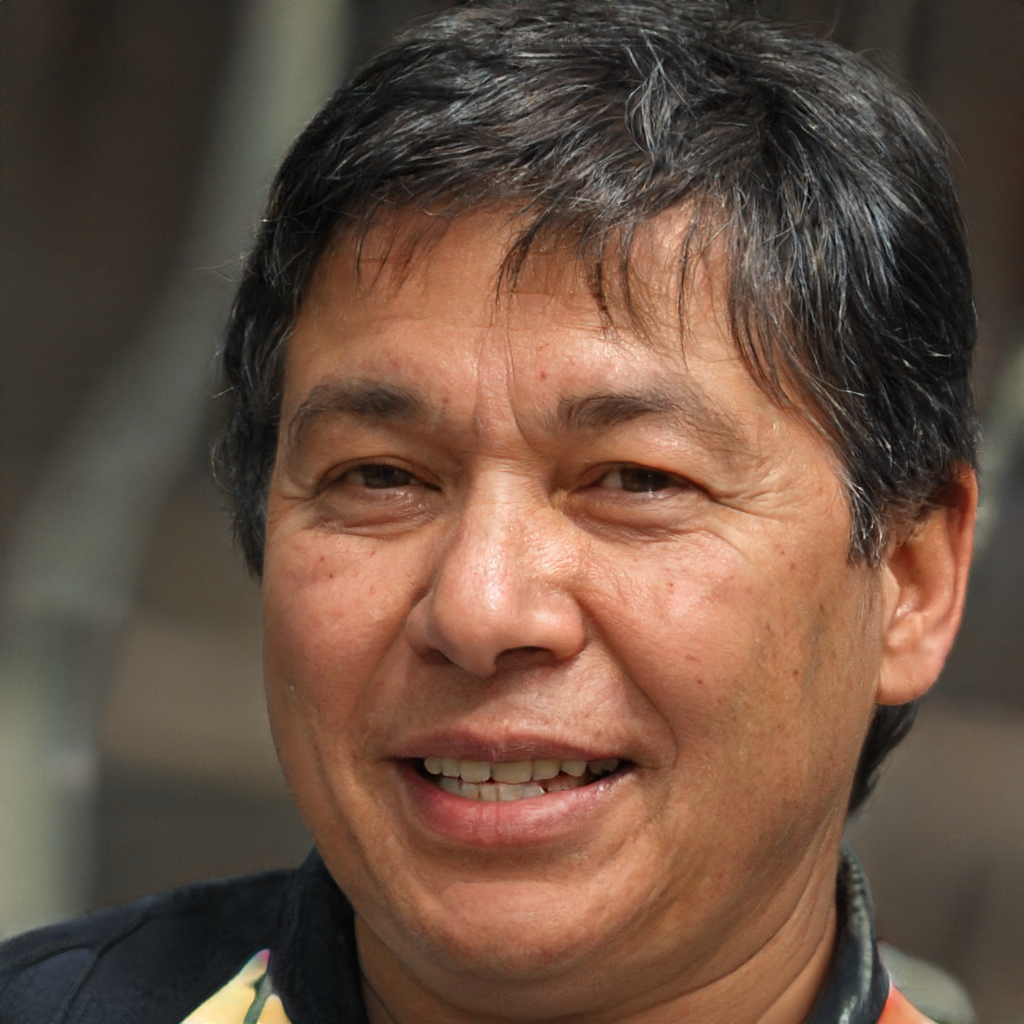
\includegraphics[scale=0.11]{persona-lee.jpg}
\end{wrapfigure}

\paragraph{Lee Henderson}

Lee recently celebrated his 50th birthday by founding his first startup. Serving in both Afghanistan and Iraq, Lee is a US Air Force veteran. Though unconventional, he decided to retire from his officer position to start a company in the aviation technology space, where he worked his entire career. 

He raised a seed round from a Silicon Valley angel investor and has began to work full-time with his recently-graduated son. Therefore, he has frequent meetings with new business partners and investors. He currently does not have any additional income apart from his army pension, but he plans on changing that soon after landing his first client.

His strength is in radio and navigation hardware technology, but still prefers to schedule appointments using pen and paper, a habit he has had since his days in the military. He is not very keen on moving to a digital system, but considers himself open-minded and likes trying new products.

\begin{table}[!htb]
	\begin{minipage}{1\linewidth}
		\caption{Comparison of User Personas}
		\centering
		\begin{tabular}{lll}
			\hline
			\textbf{User} & \textbf{Income} & \textbf{Requirement}         \\
			\hline
			Tanya         & Low             & Appointments with professors \\
			Julia         & Medium          & Managing time slots          \\
			Joy           & High            & Calls with team              \\
			Lee           & Medium          & Meetings with partners       \\
			\hline
		\end{tabular}
	\end{minipage}%
\end{table}

Though the use cases for each persona are different, they all fall under the umbrella of ``I want a better, more automated way of scheduling appointments." For Tanya, it is to interact with professors; for Julia, with clients; for Joy, with her team; and for Lee, with his business partners. With an automated virtual agent that can schedule appointments without input from users, a significant part of all of their problems may be solved.

\subsection{Assistant Architecture}

An exploration of the the entire process from receiving a new email, understanding it, and performing an action, was conducted.

\begin{wrapfigure}{l}{0.5\textwidth}\centering
	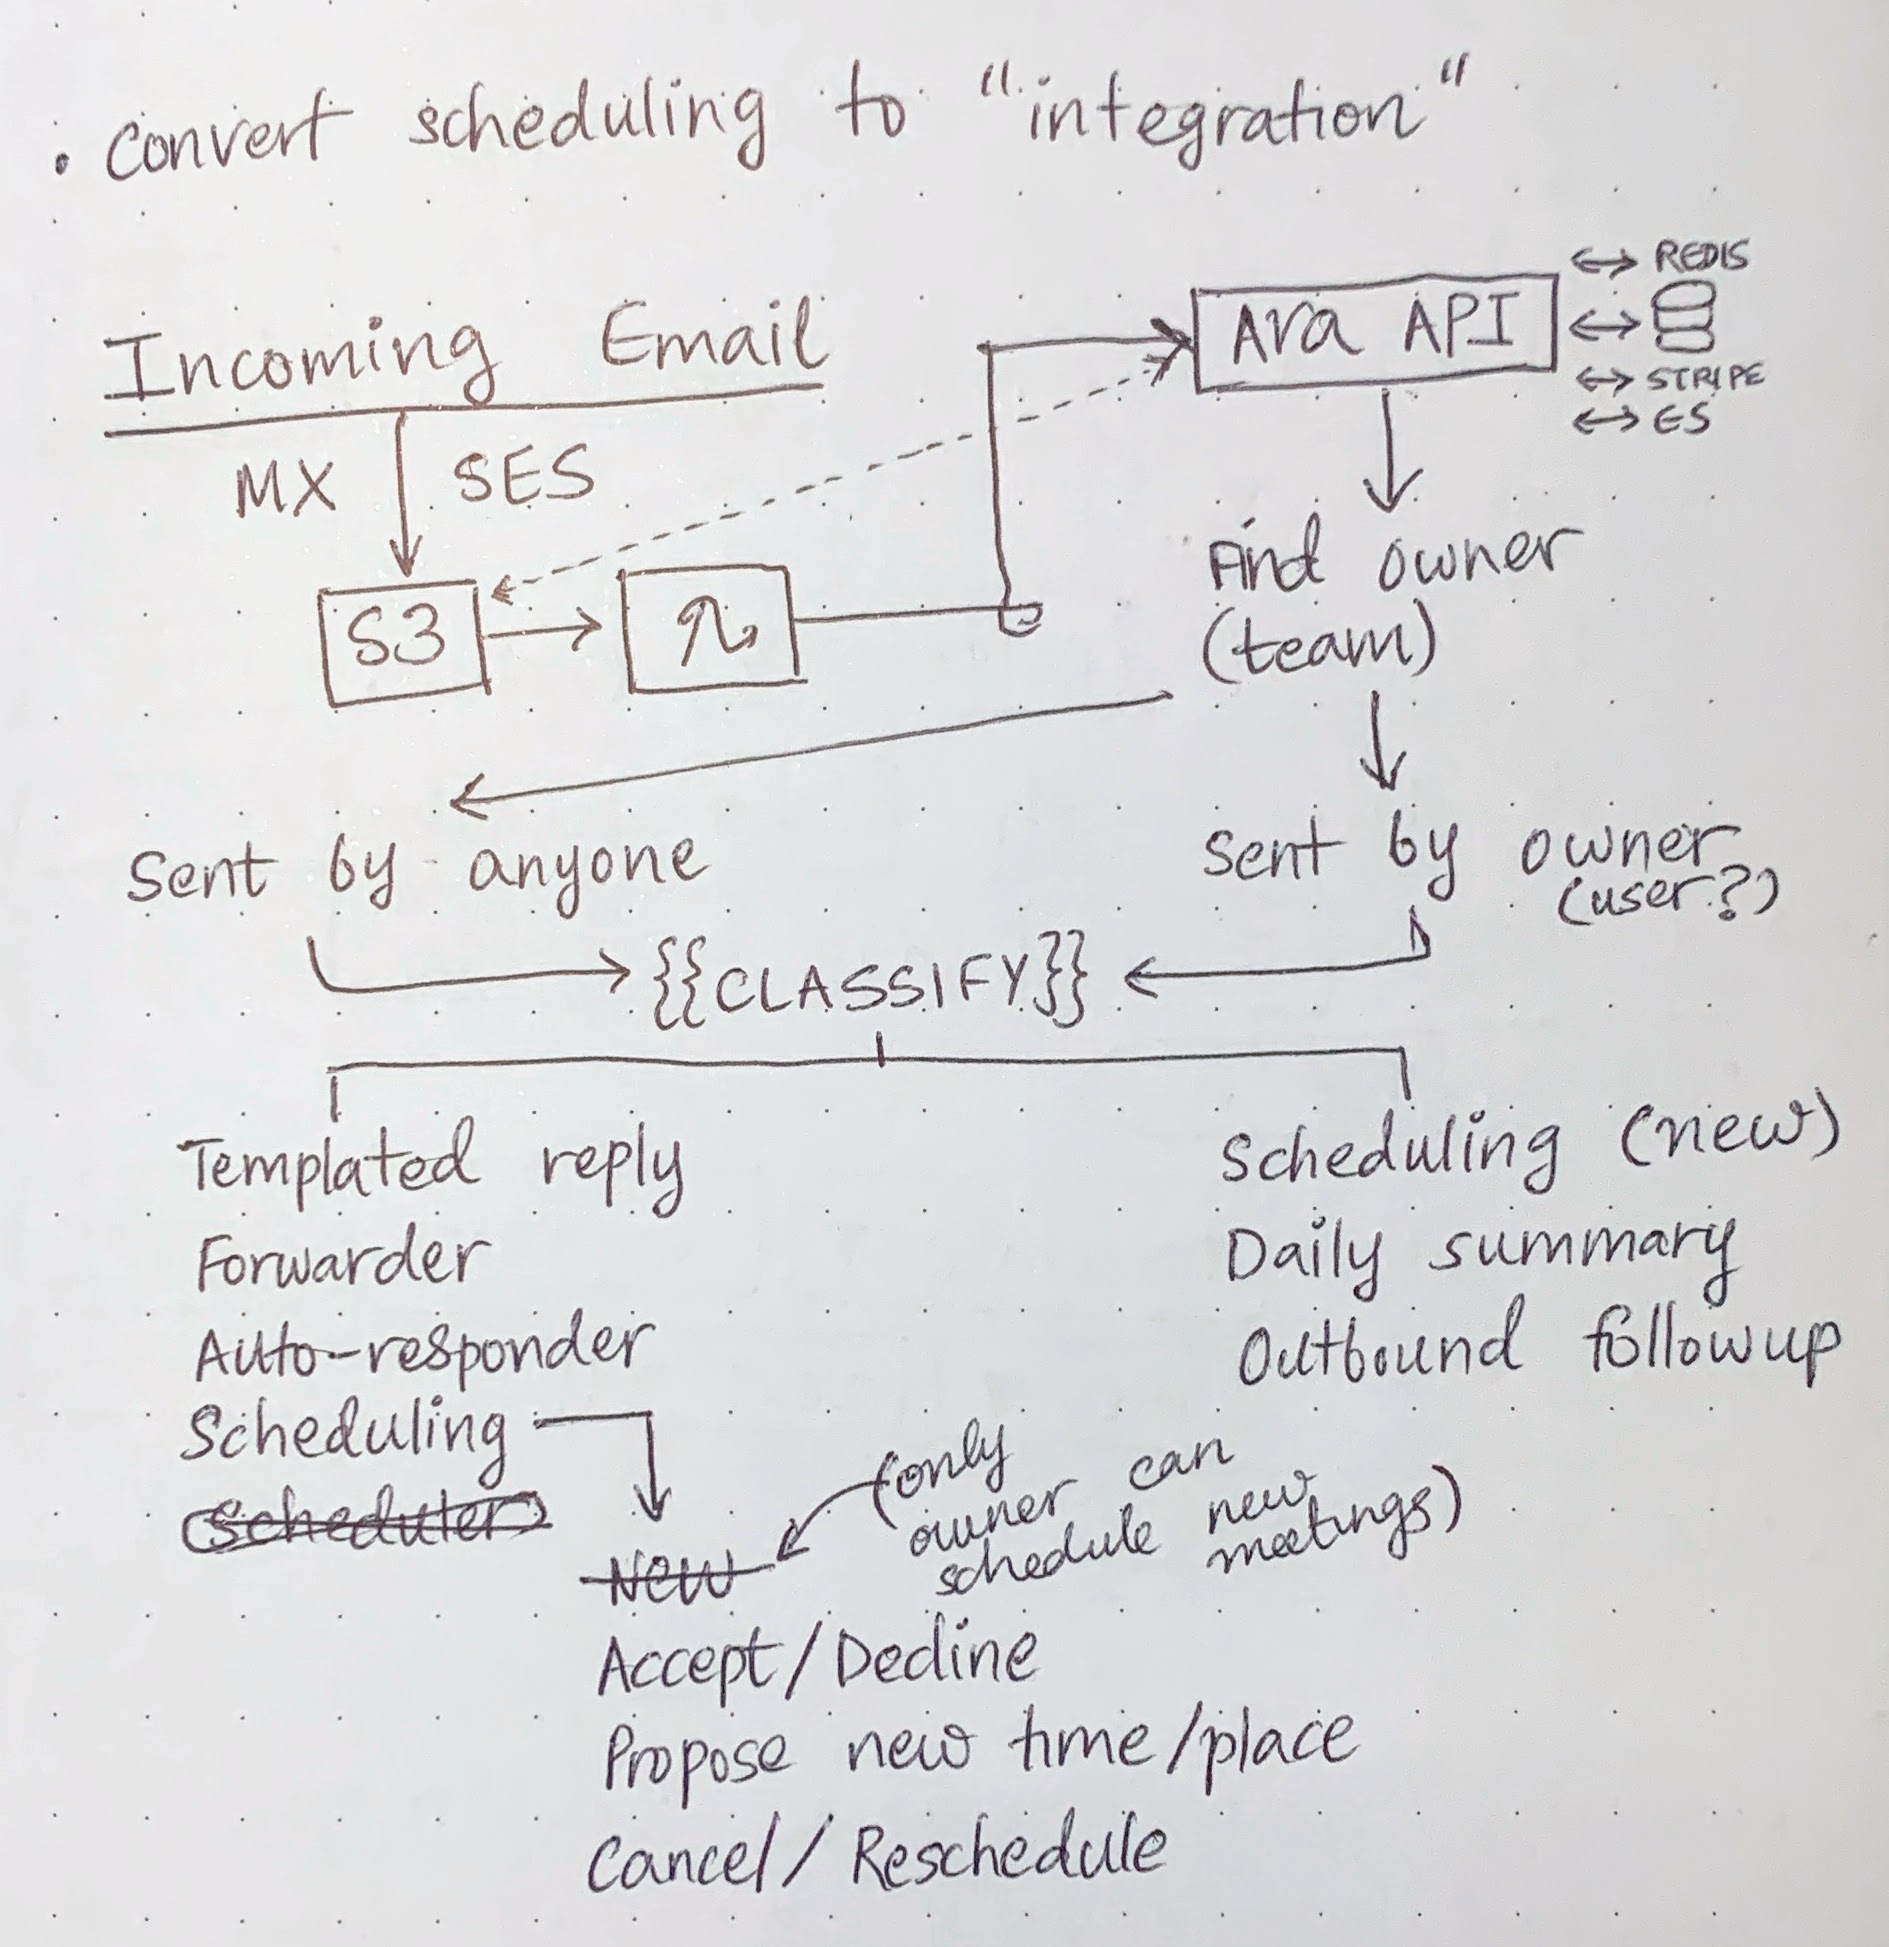
\includegraphics[scale=0.097]{drawing-all-process.jpg}
	\caption{Email process ideation}
\end{wrapfigure}

In Figure 1, the each intent (such as scheduling an appointment, forwarding an email, etc.), is performed based on the classification of the incoming email. The process assumes that incoming emails are accepted using mail exchanger (MX) records pointed to Amazon Web Services (AWS)'s Simple Email Service (SES) [rfc2181]. This was decided based on literature research (Section 2.2).

Then, the incoming email is saved in an S3 bucket and a Lambda serverless function is invoked that triggers the API. The diagram also showcases the connection of the API with other services like a database, Redis, Stripe, and ElasticSearch.

The API then finds the owner of the team the email was addressed to and whether or not the owner themselves sent the email. After classification, one of several processes are queued.

\begin{wrapfigure}{r}{0.5\textwidth}\centering
	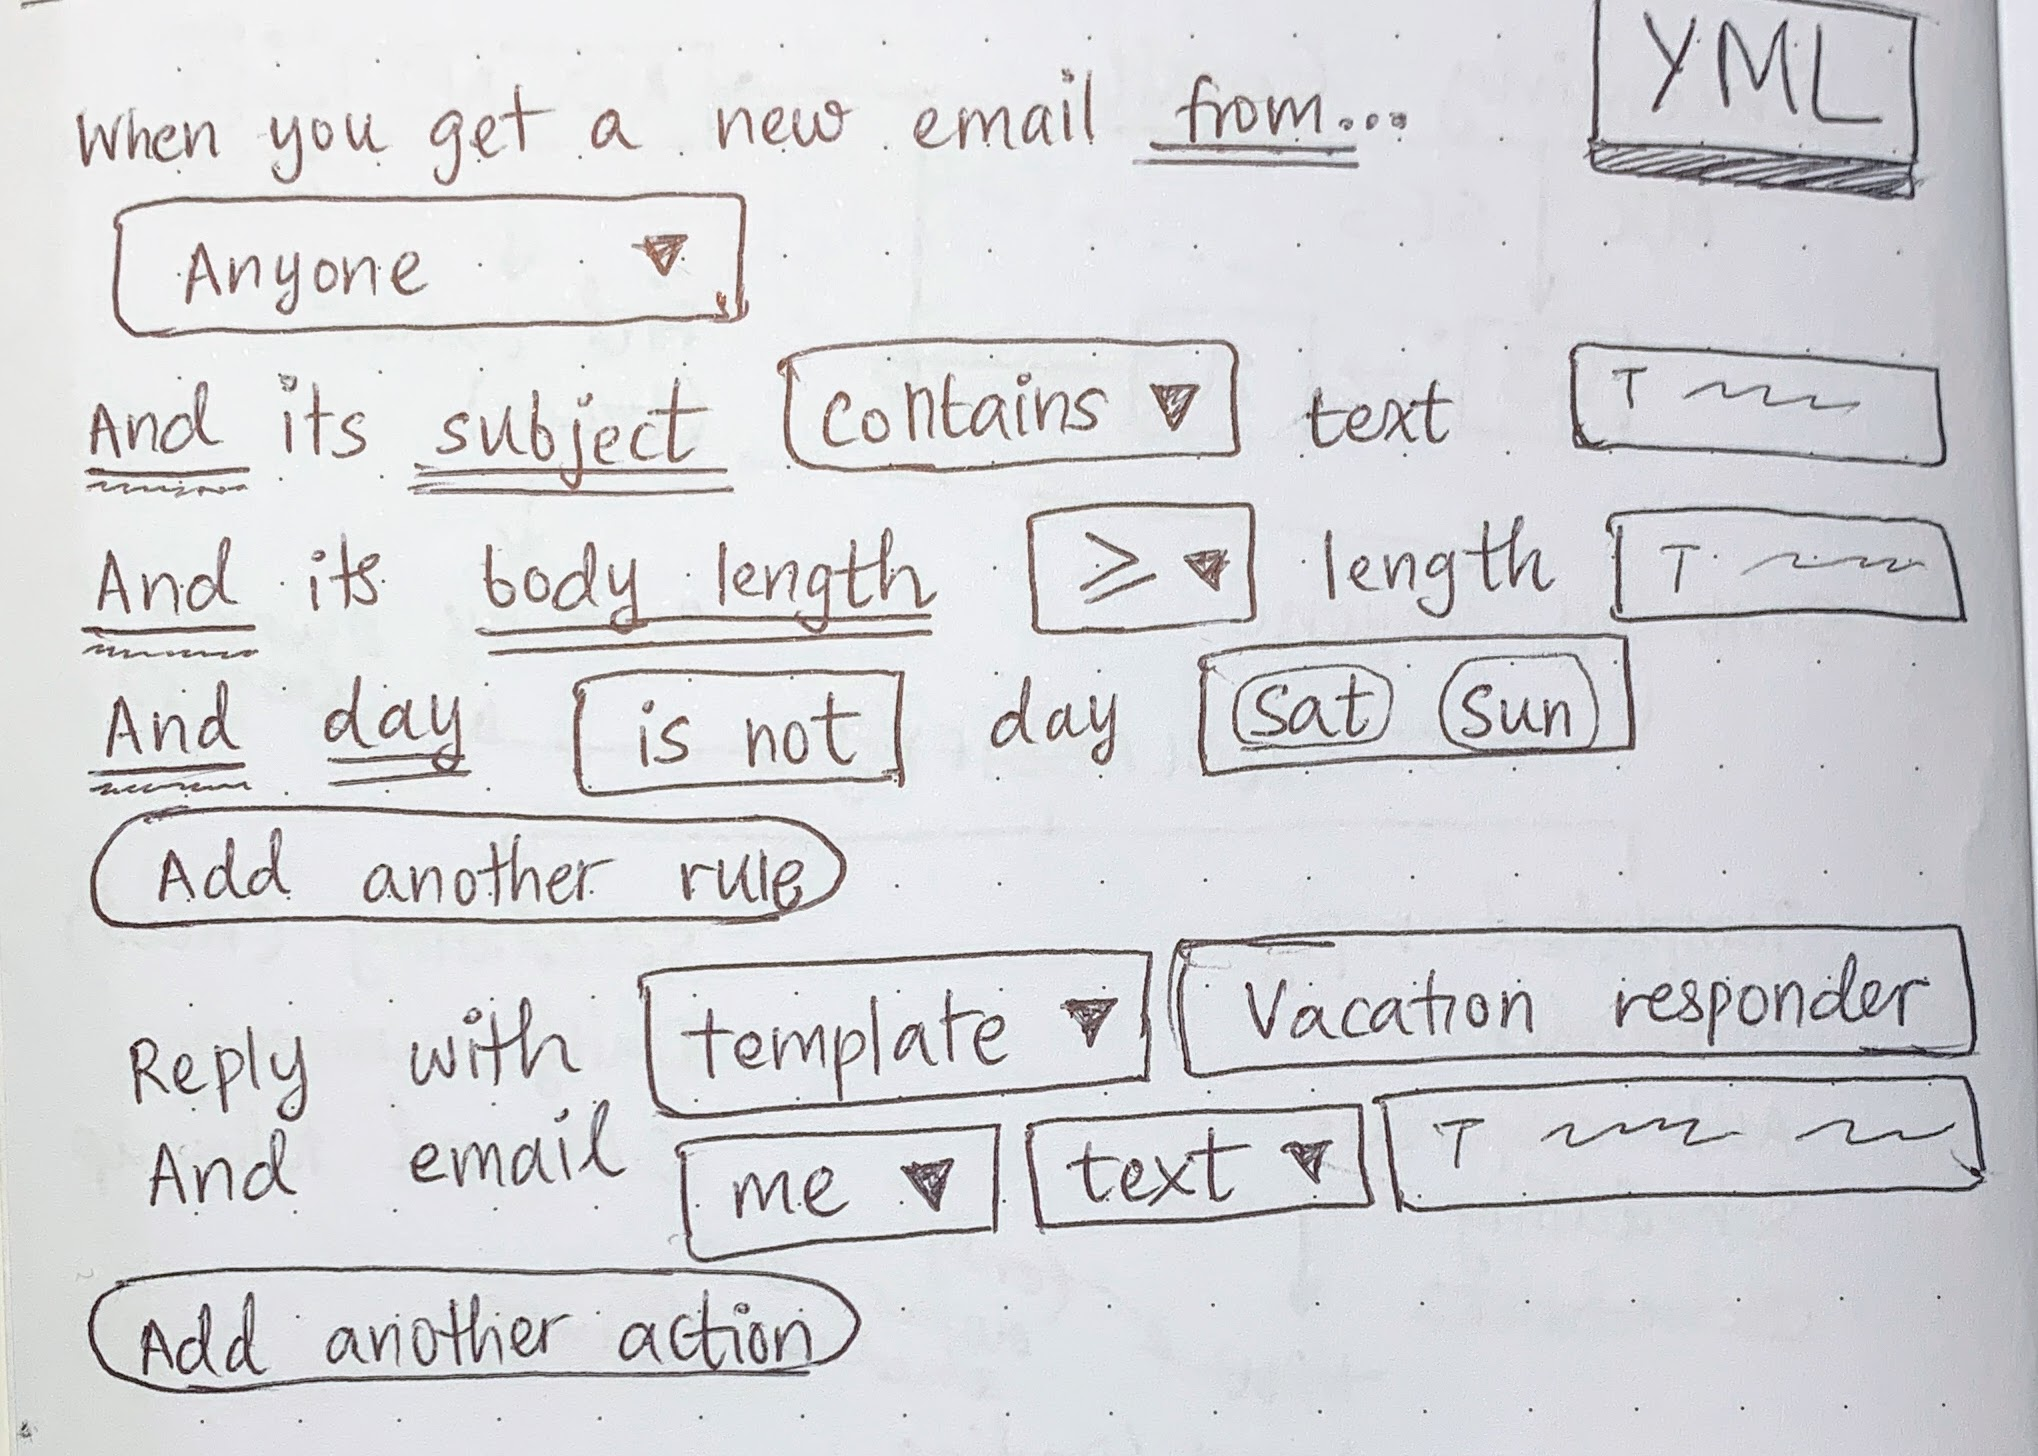
\includegraphics[scale=0.092]{drawing-rules-ui.jpg}
	\caption{Rule-based process ideation}
\end{wrapfigure}

In a separate exploration, a rule-based approach was chosen rather than specific tasks that the assistant can perform. In Figure 2, a user interface was mocked up wherein consumers could set custom rules to perform action when new emails are received. In the example, there are three types of UI elements --- select dropdowns, text inputs, and buttons.

In the example UI, the rule is "When you get an email from \emph{anyone}, \emph{and} its \emph{subject} \emph{contains} the text (input), \emph{and} its \emph{body length} \emph{is greater than or equal to} (length), \emph{and} the \emph{day} \emph{is not} one of the days \emph{Sat, Sun}, automatically reply with \emph{template} \emph{Vacation responder} and also email \emph{me} with the (text). Complicated rules such as these can be generated by the proposed UI, allowing users to automate several different types of repetitive email tasks.

\subsection{Web App UI}

...text...

\begin{figure}
  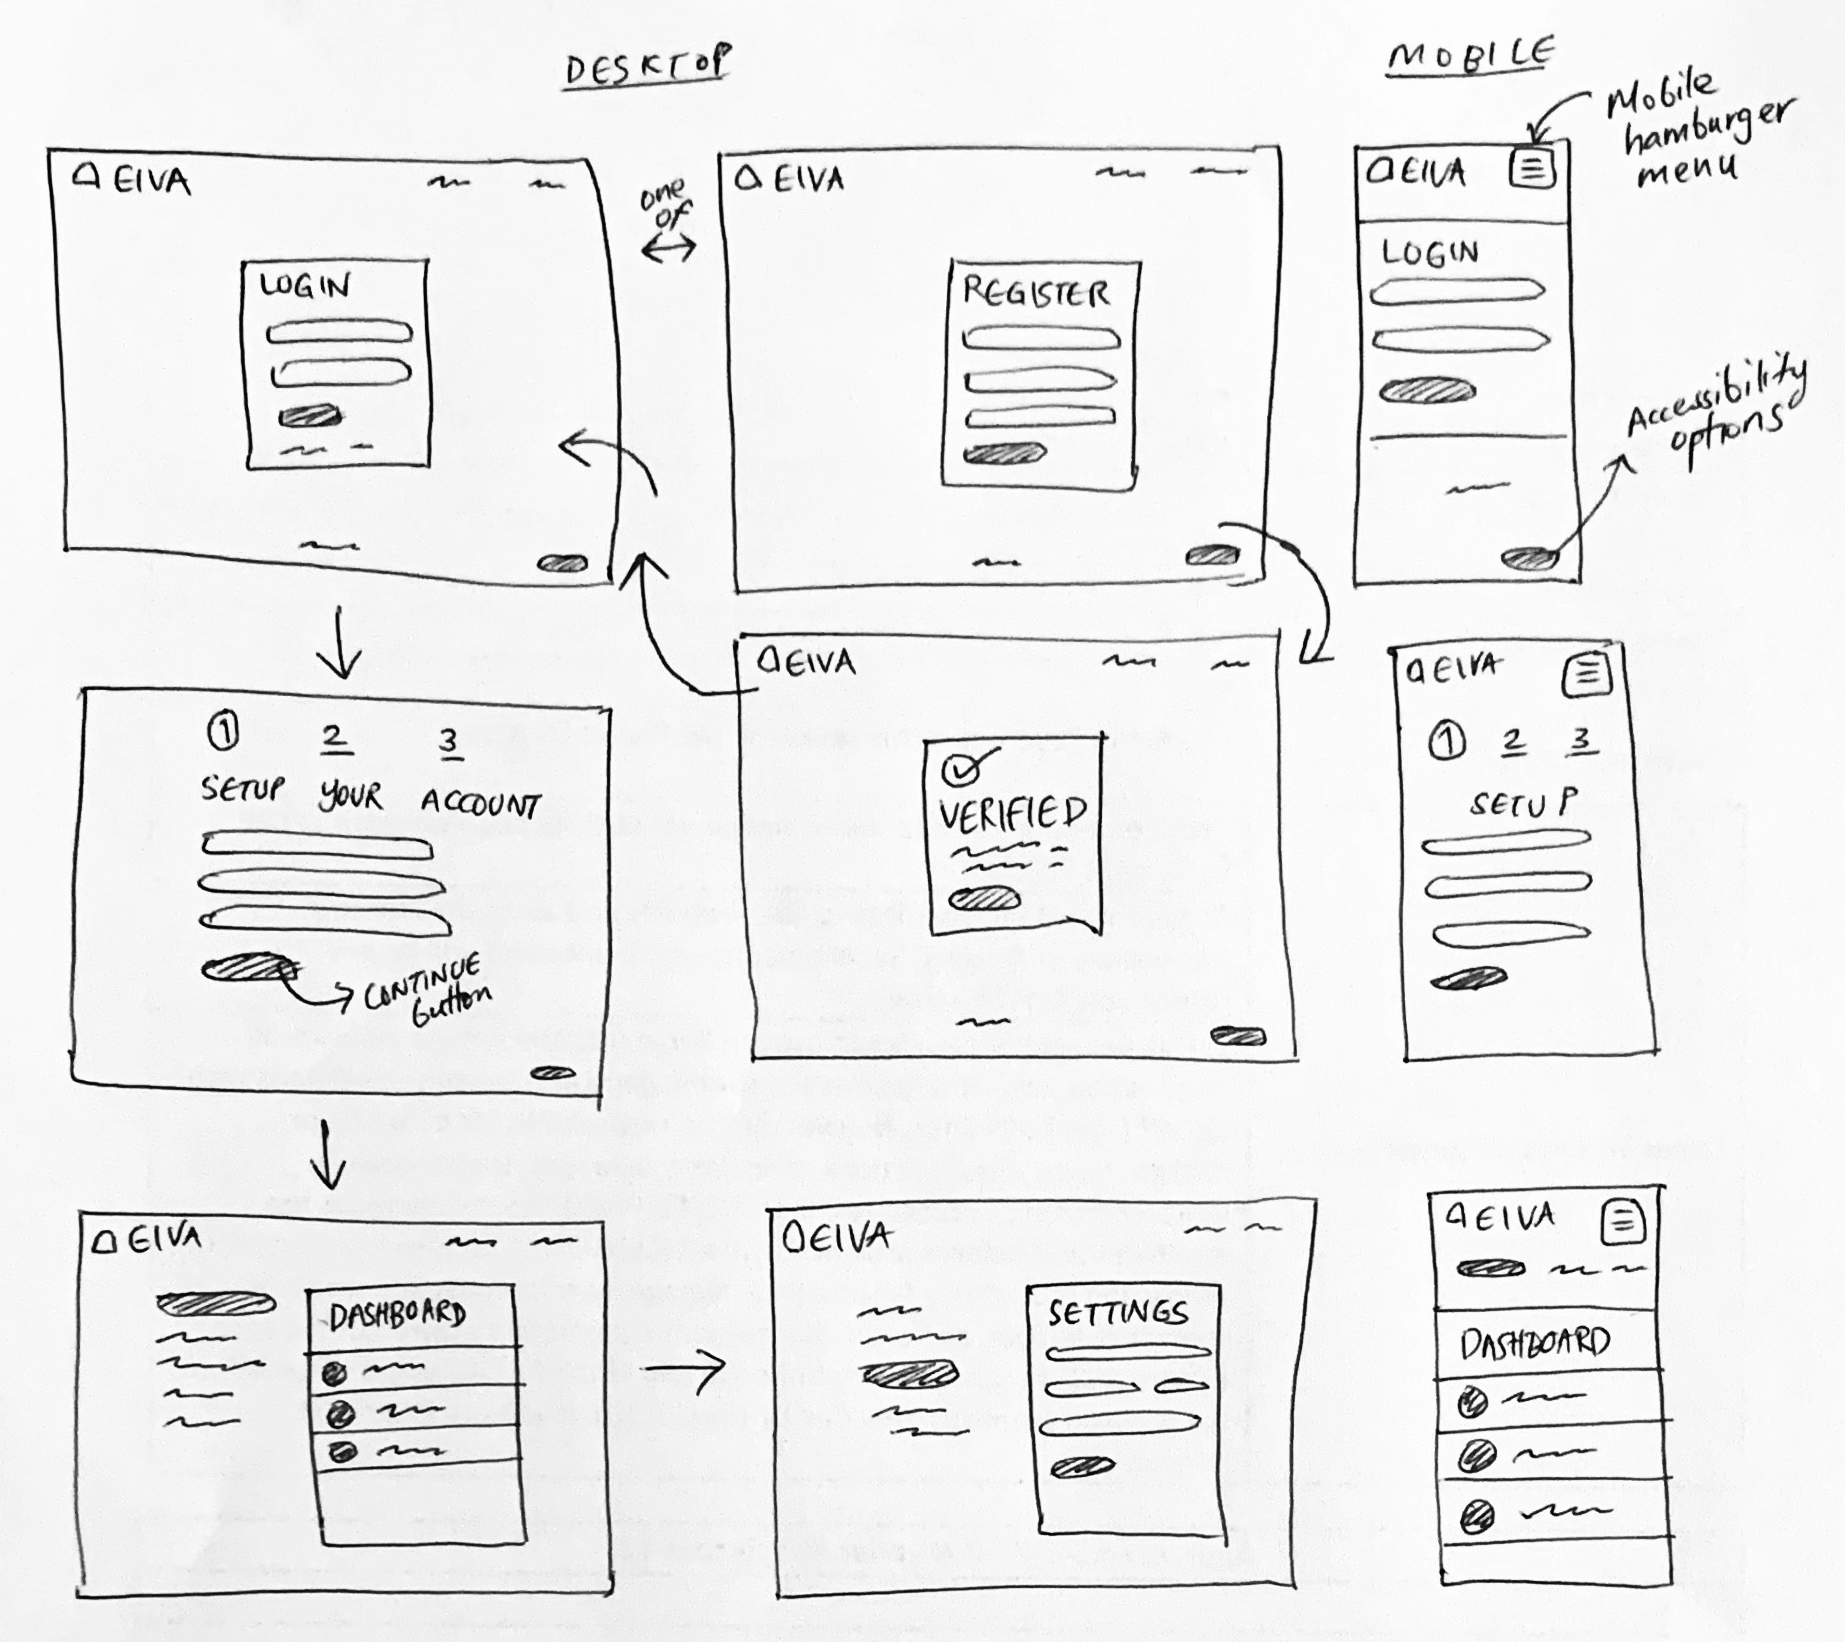
\includegraphics[width=\textwidth]{drawing-ui.jpg}
  \caption{Webpage Wireframes on Paper}
\end{figure}

...text...

\begin{figure}
  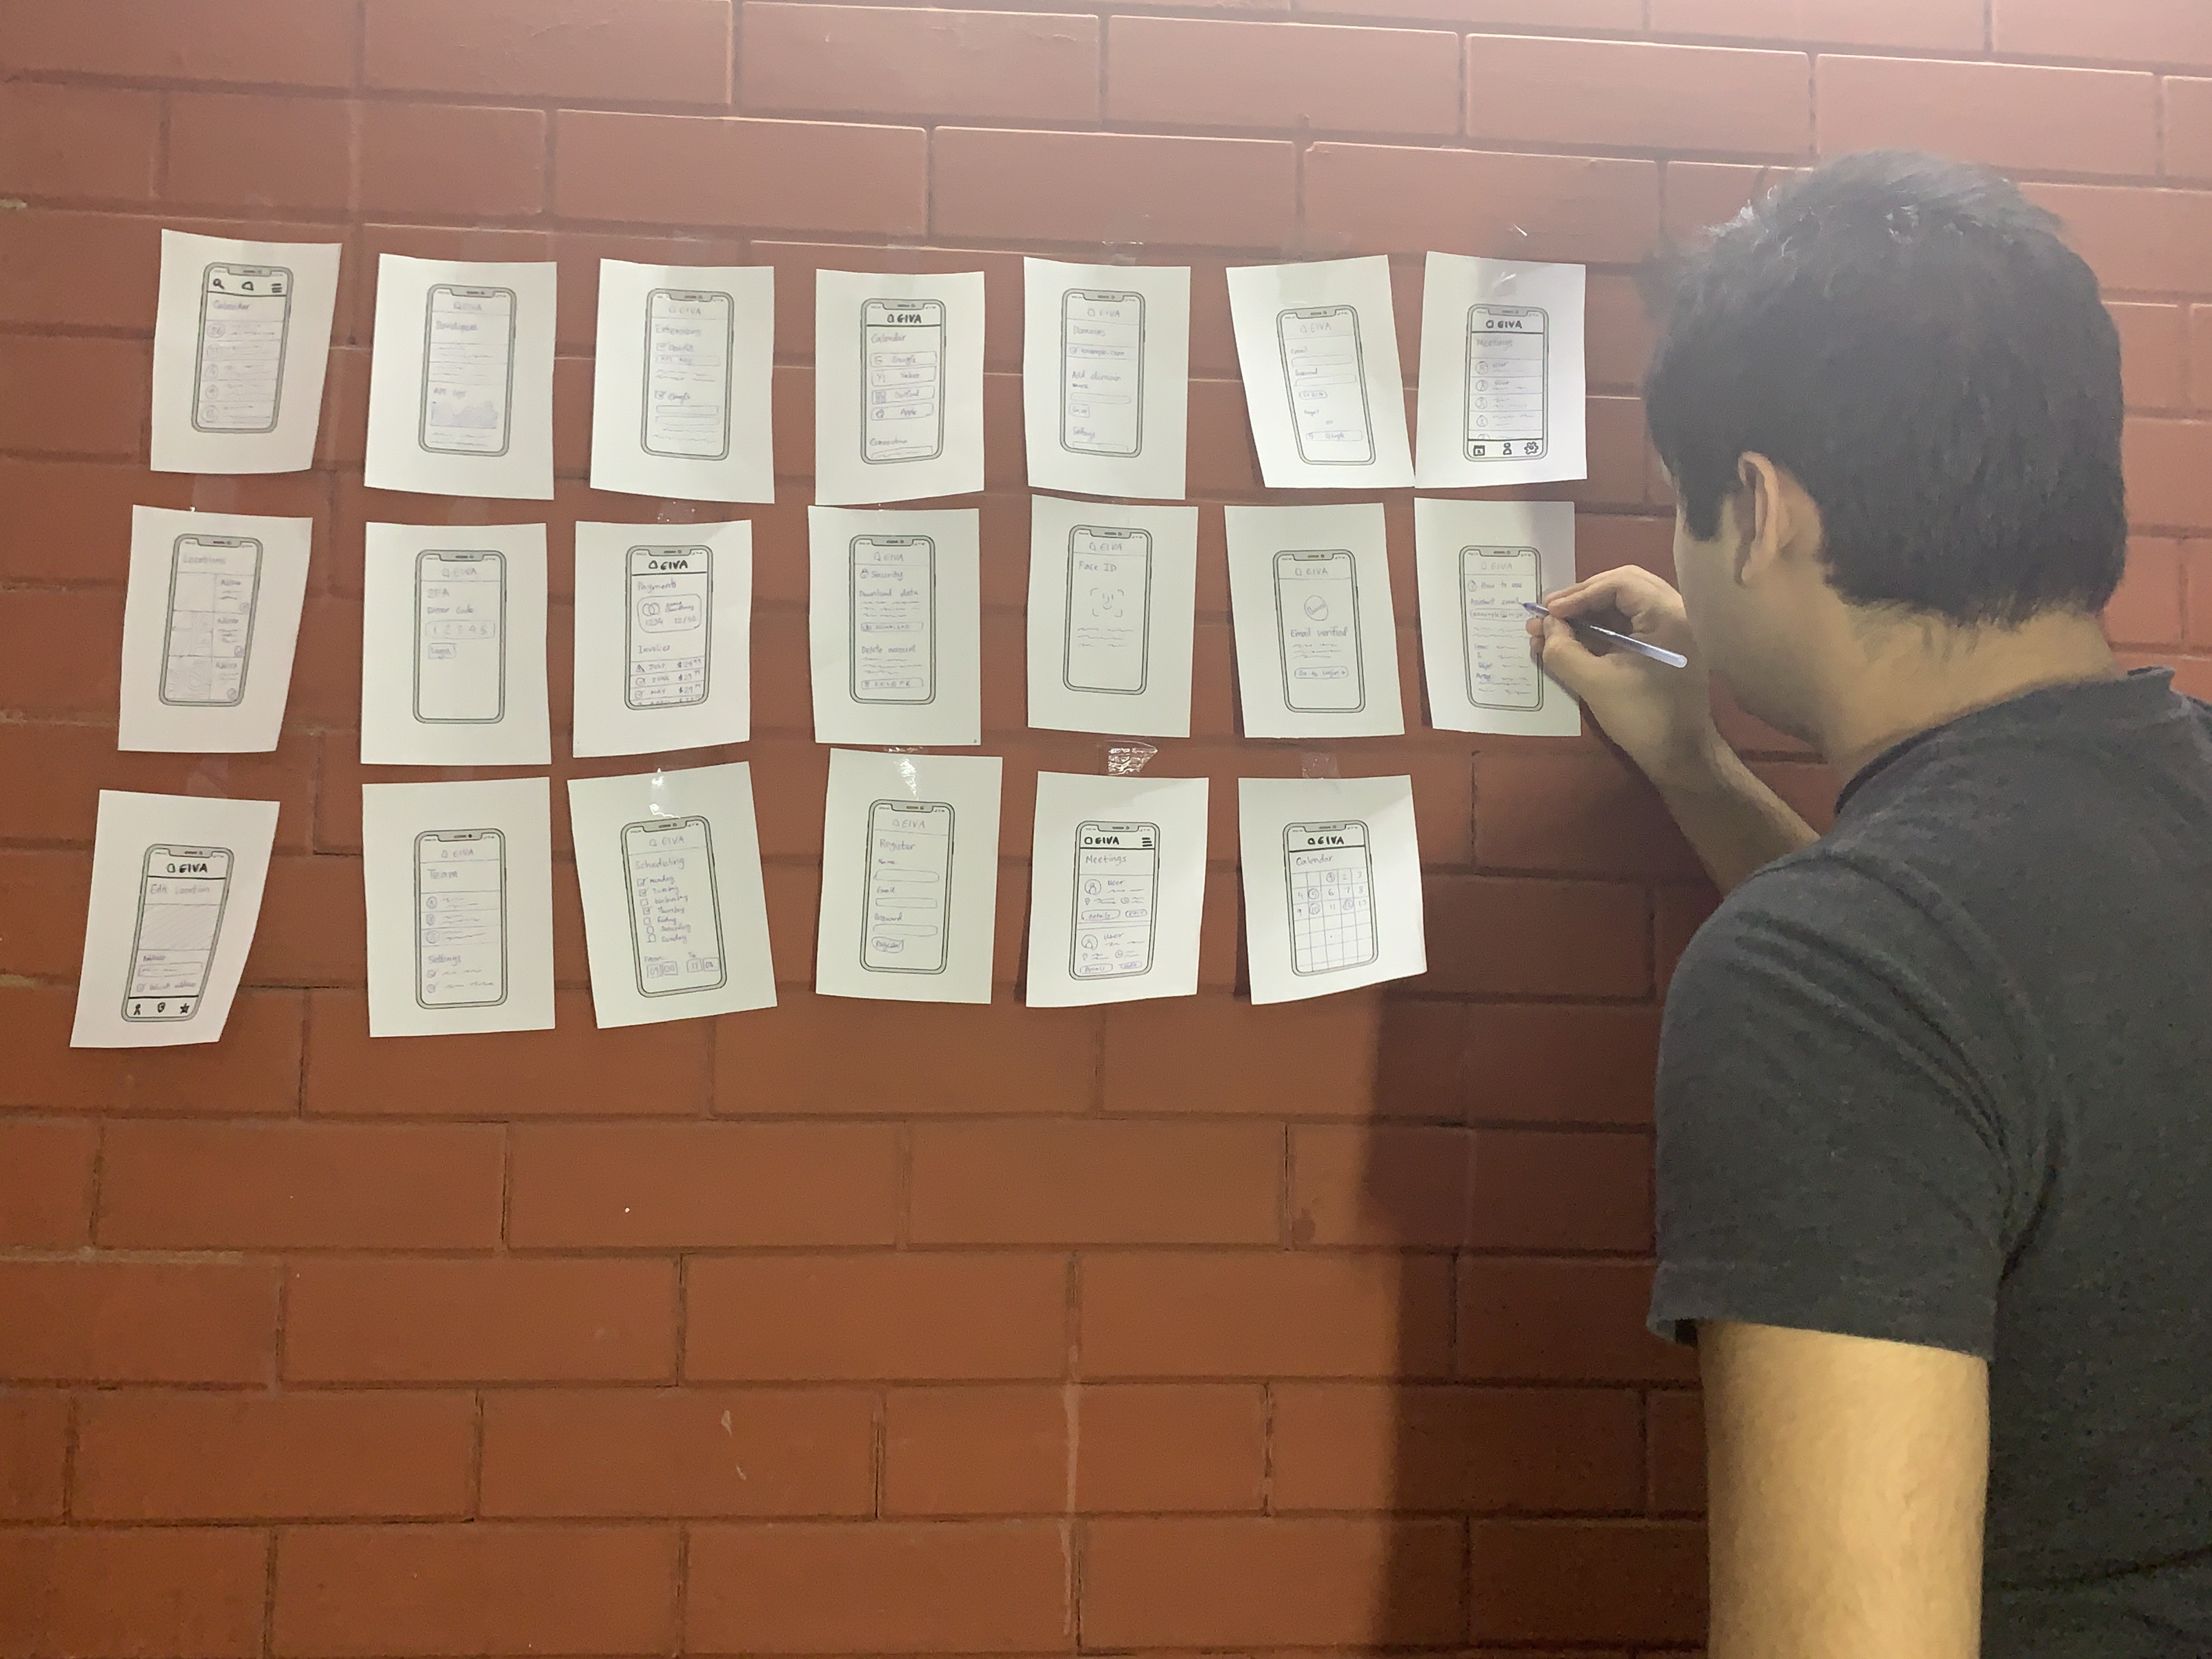
\includegraphics[width=\textwidth]{ideation-wall.jpg}
  \caption{Mobile Wireframes Exploration}
\end{figure}

...text...

\begin{figure}
	\centering
	\begin{minipage}{.5\textwidth}
		\centering
		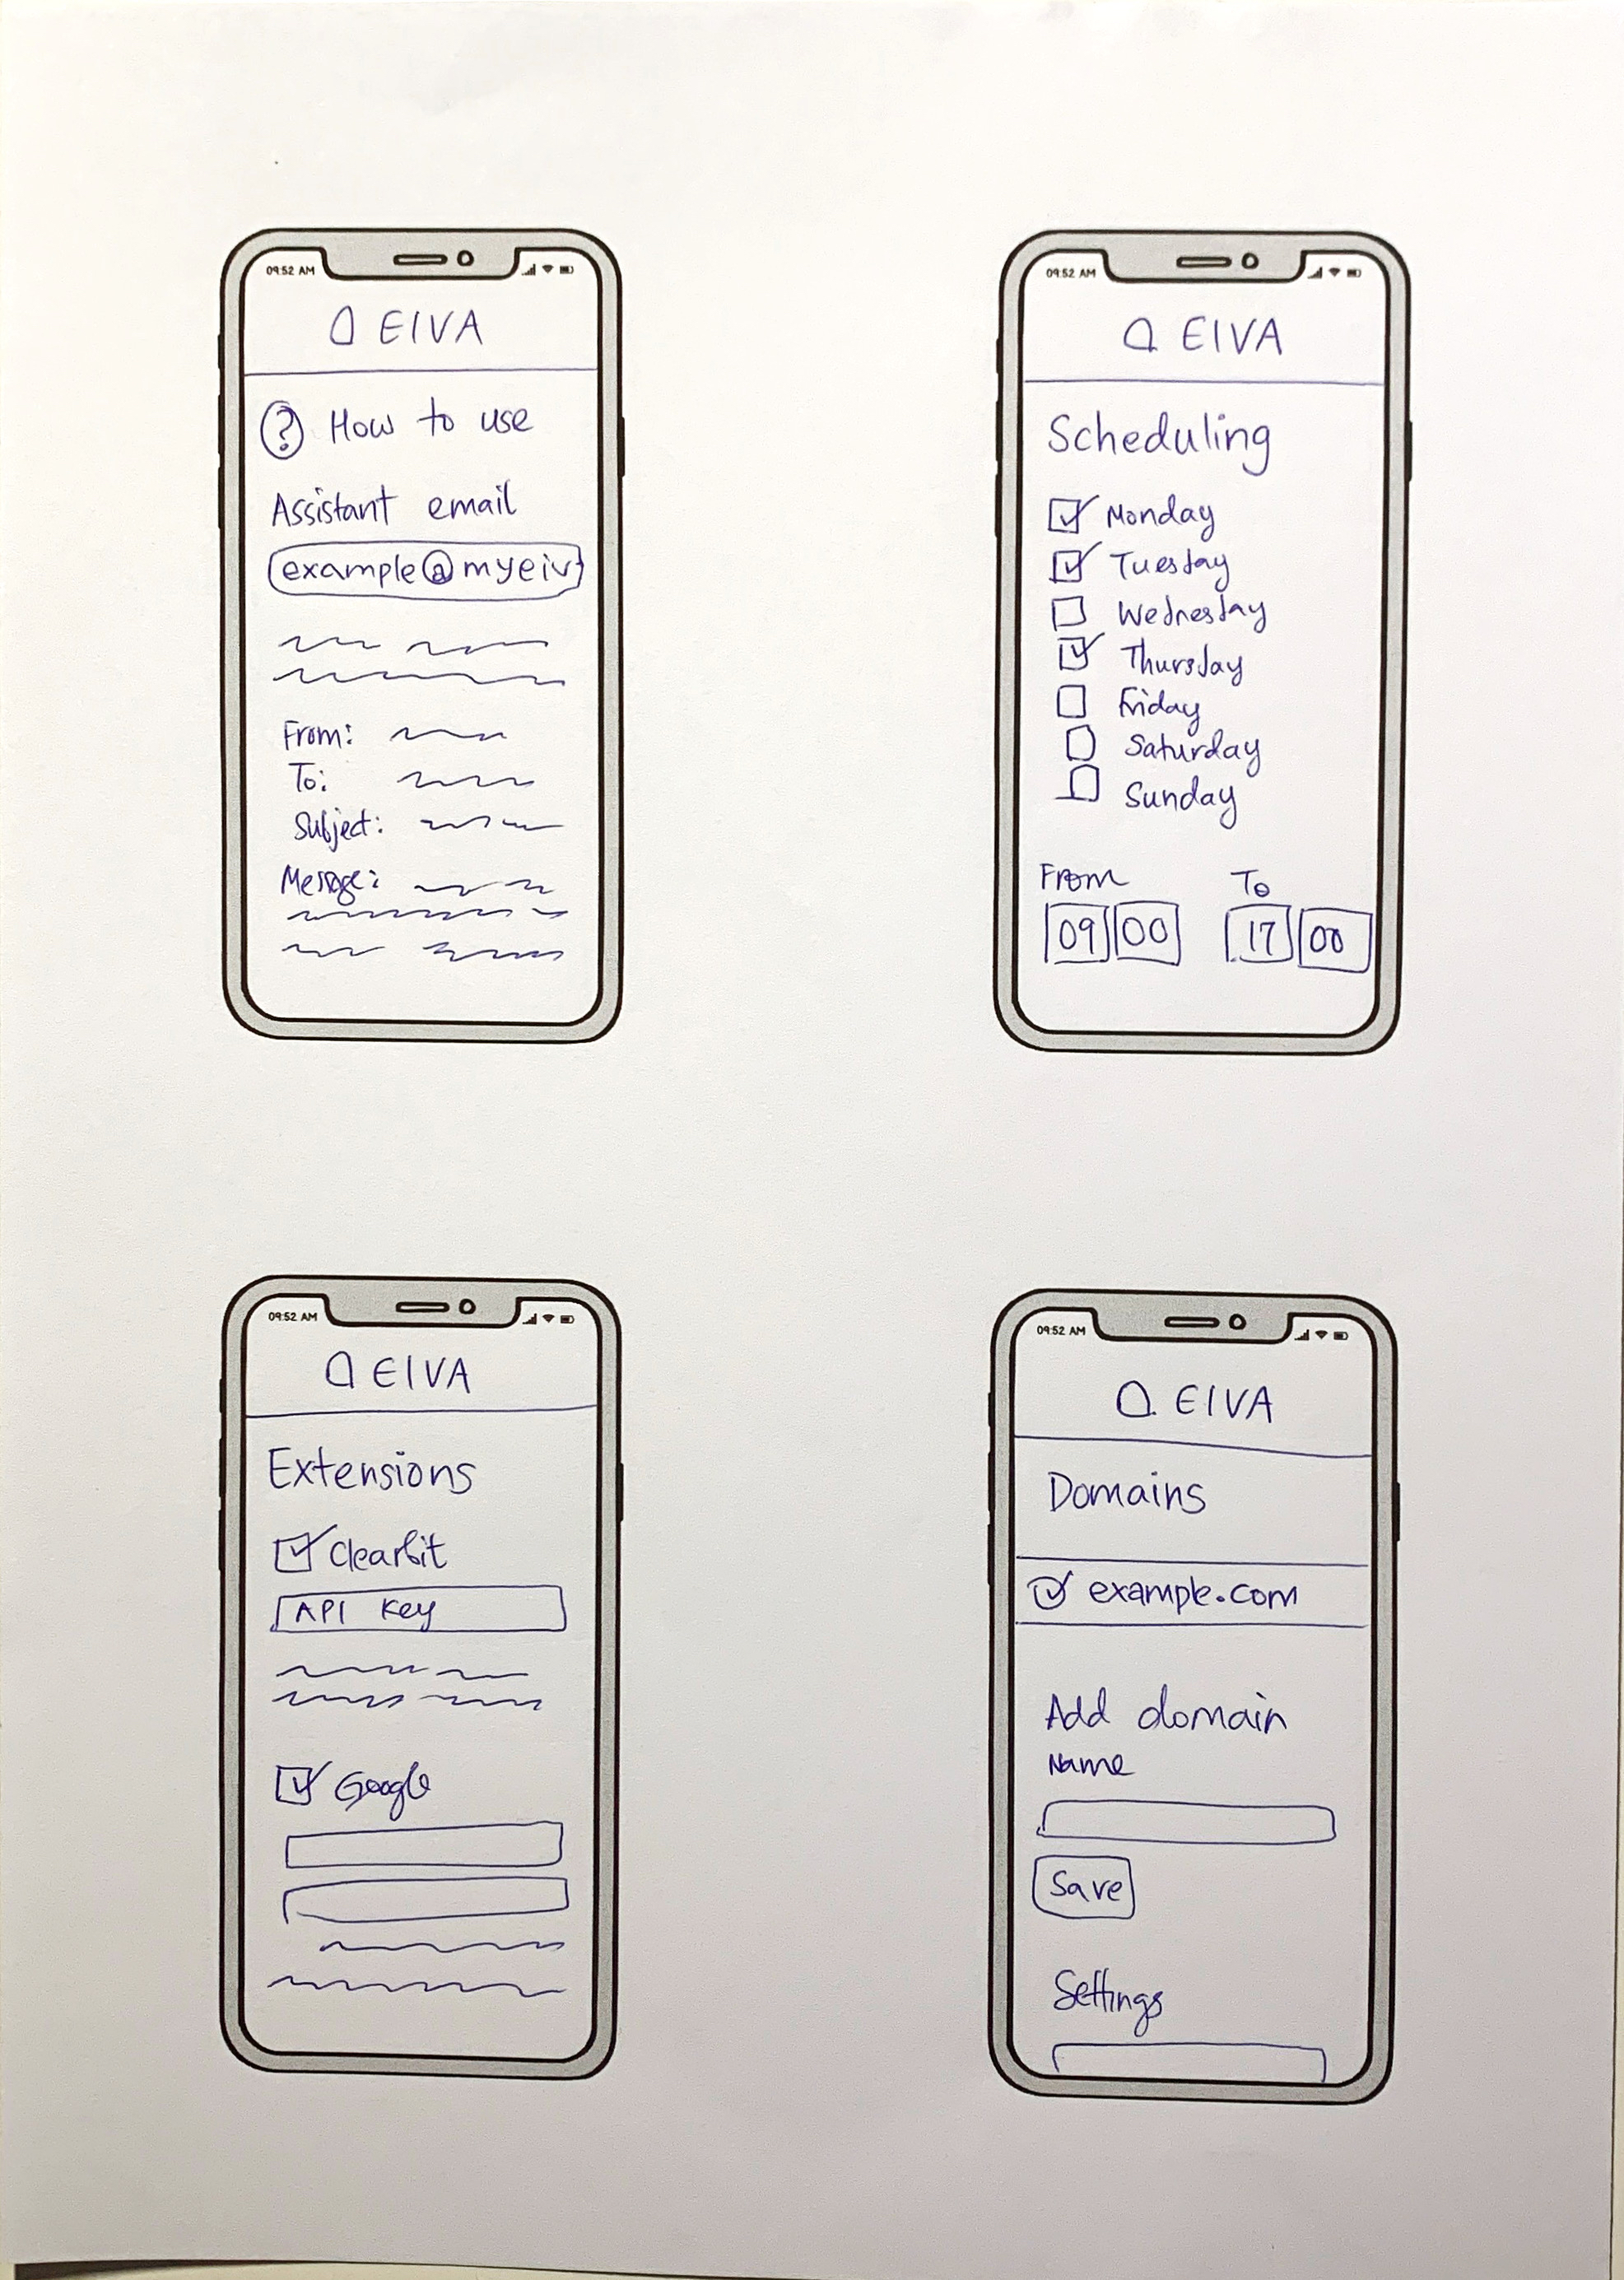
\includegraphics[width=1\linewidth]{drawing-phone-1.jpg}
		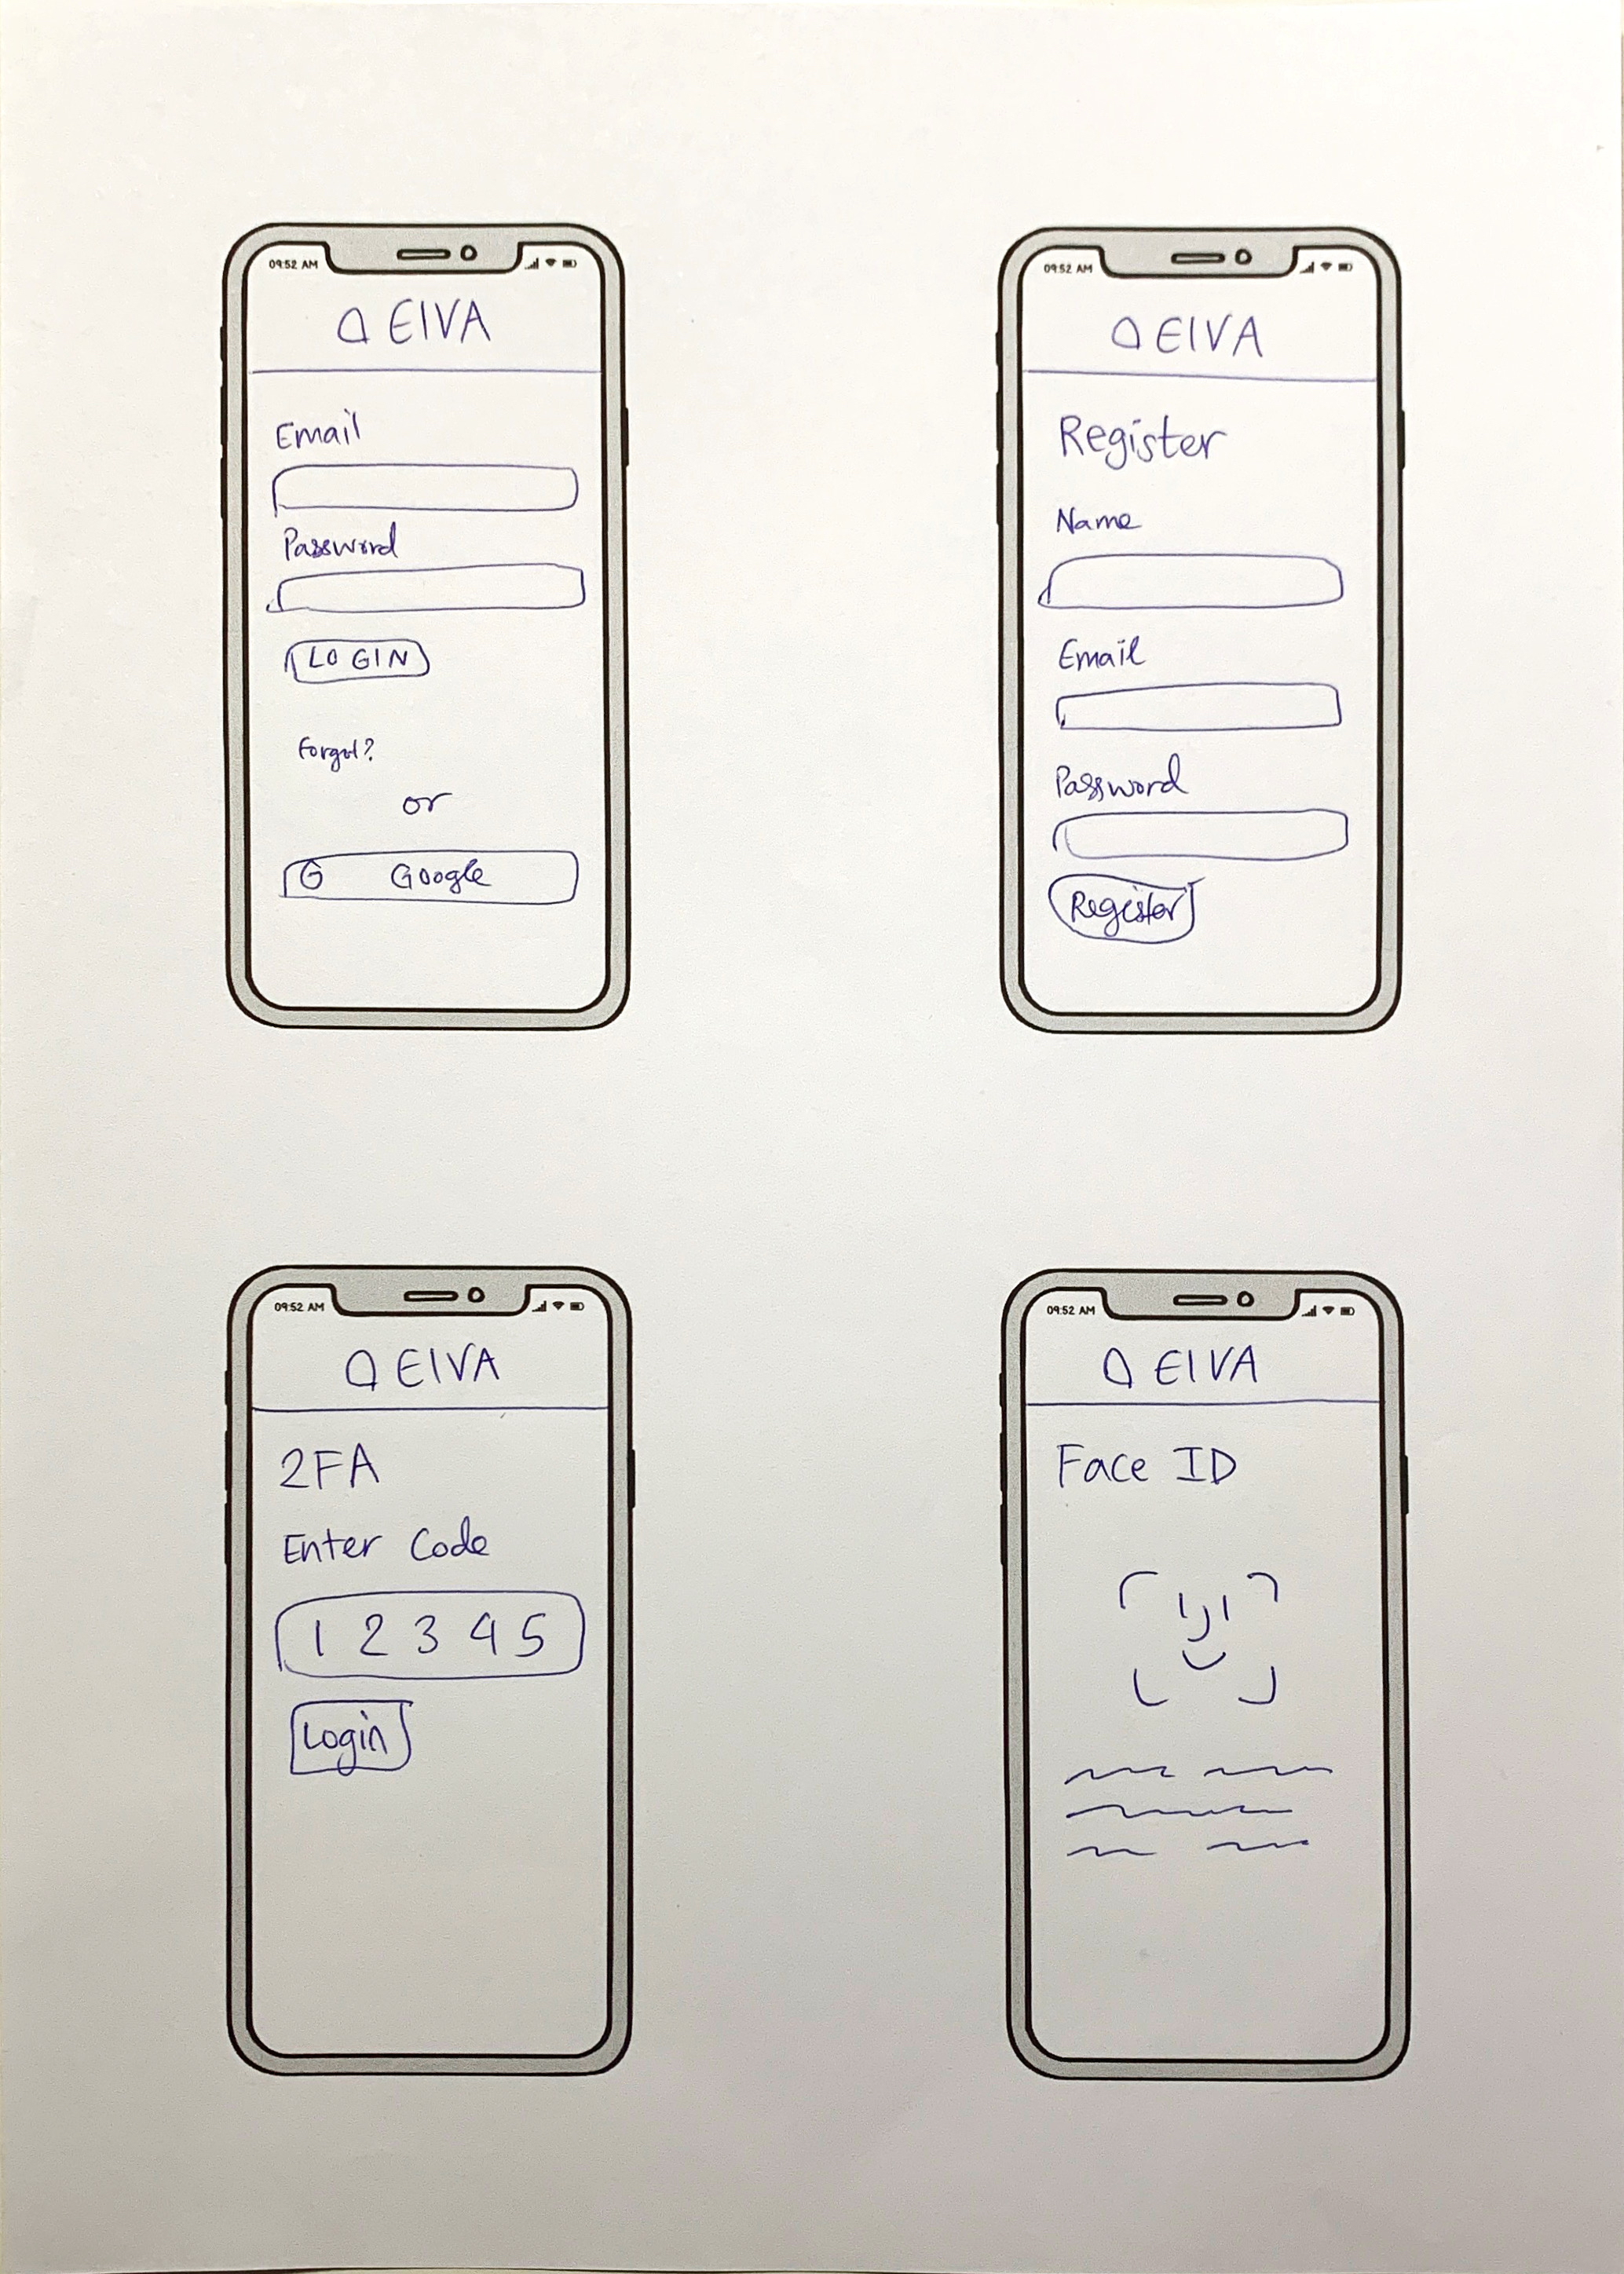
\includegraphics[width=1\linewidth]{drawing-phone-2.jpg}
	\end{minipage}%
	\begin{minipage}{.5\textwidth}
		\centering
		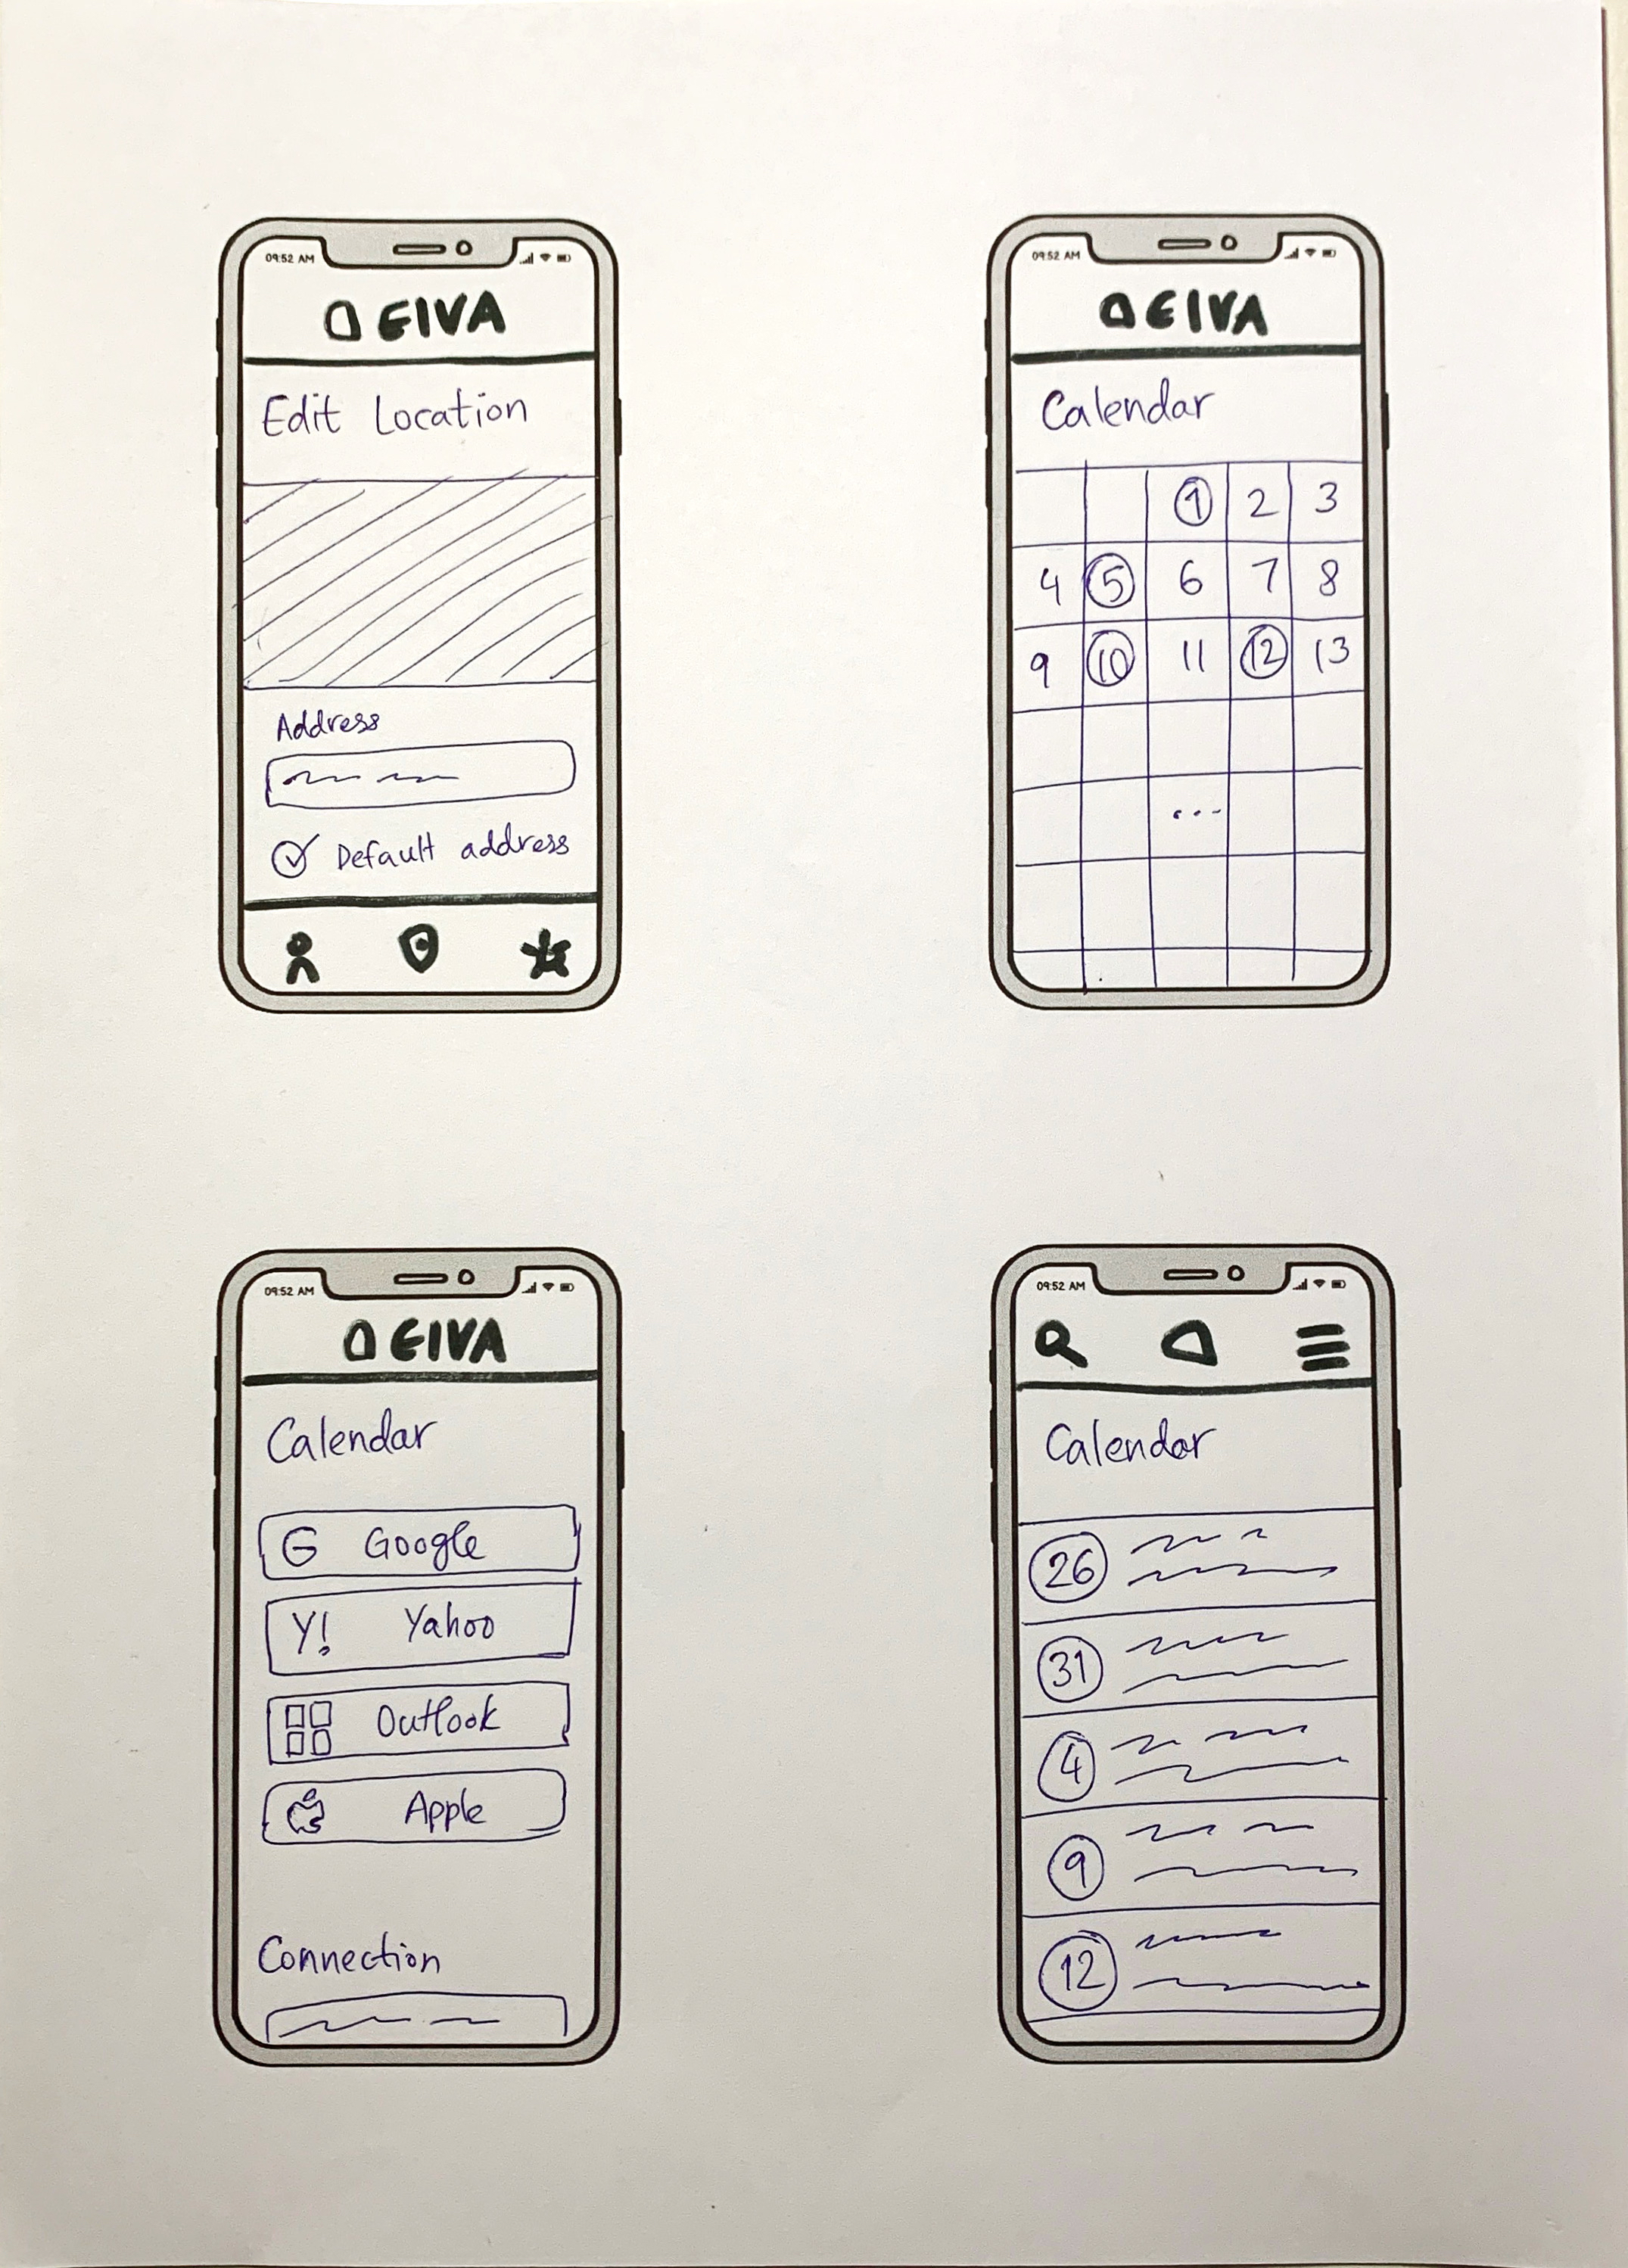
\includegraphics[width=1\linewidth]{drawing-phone-3.jpg}
		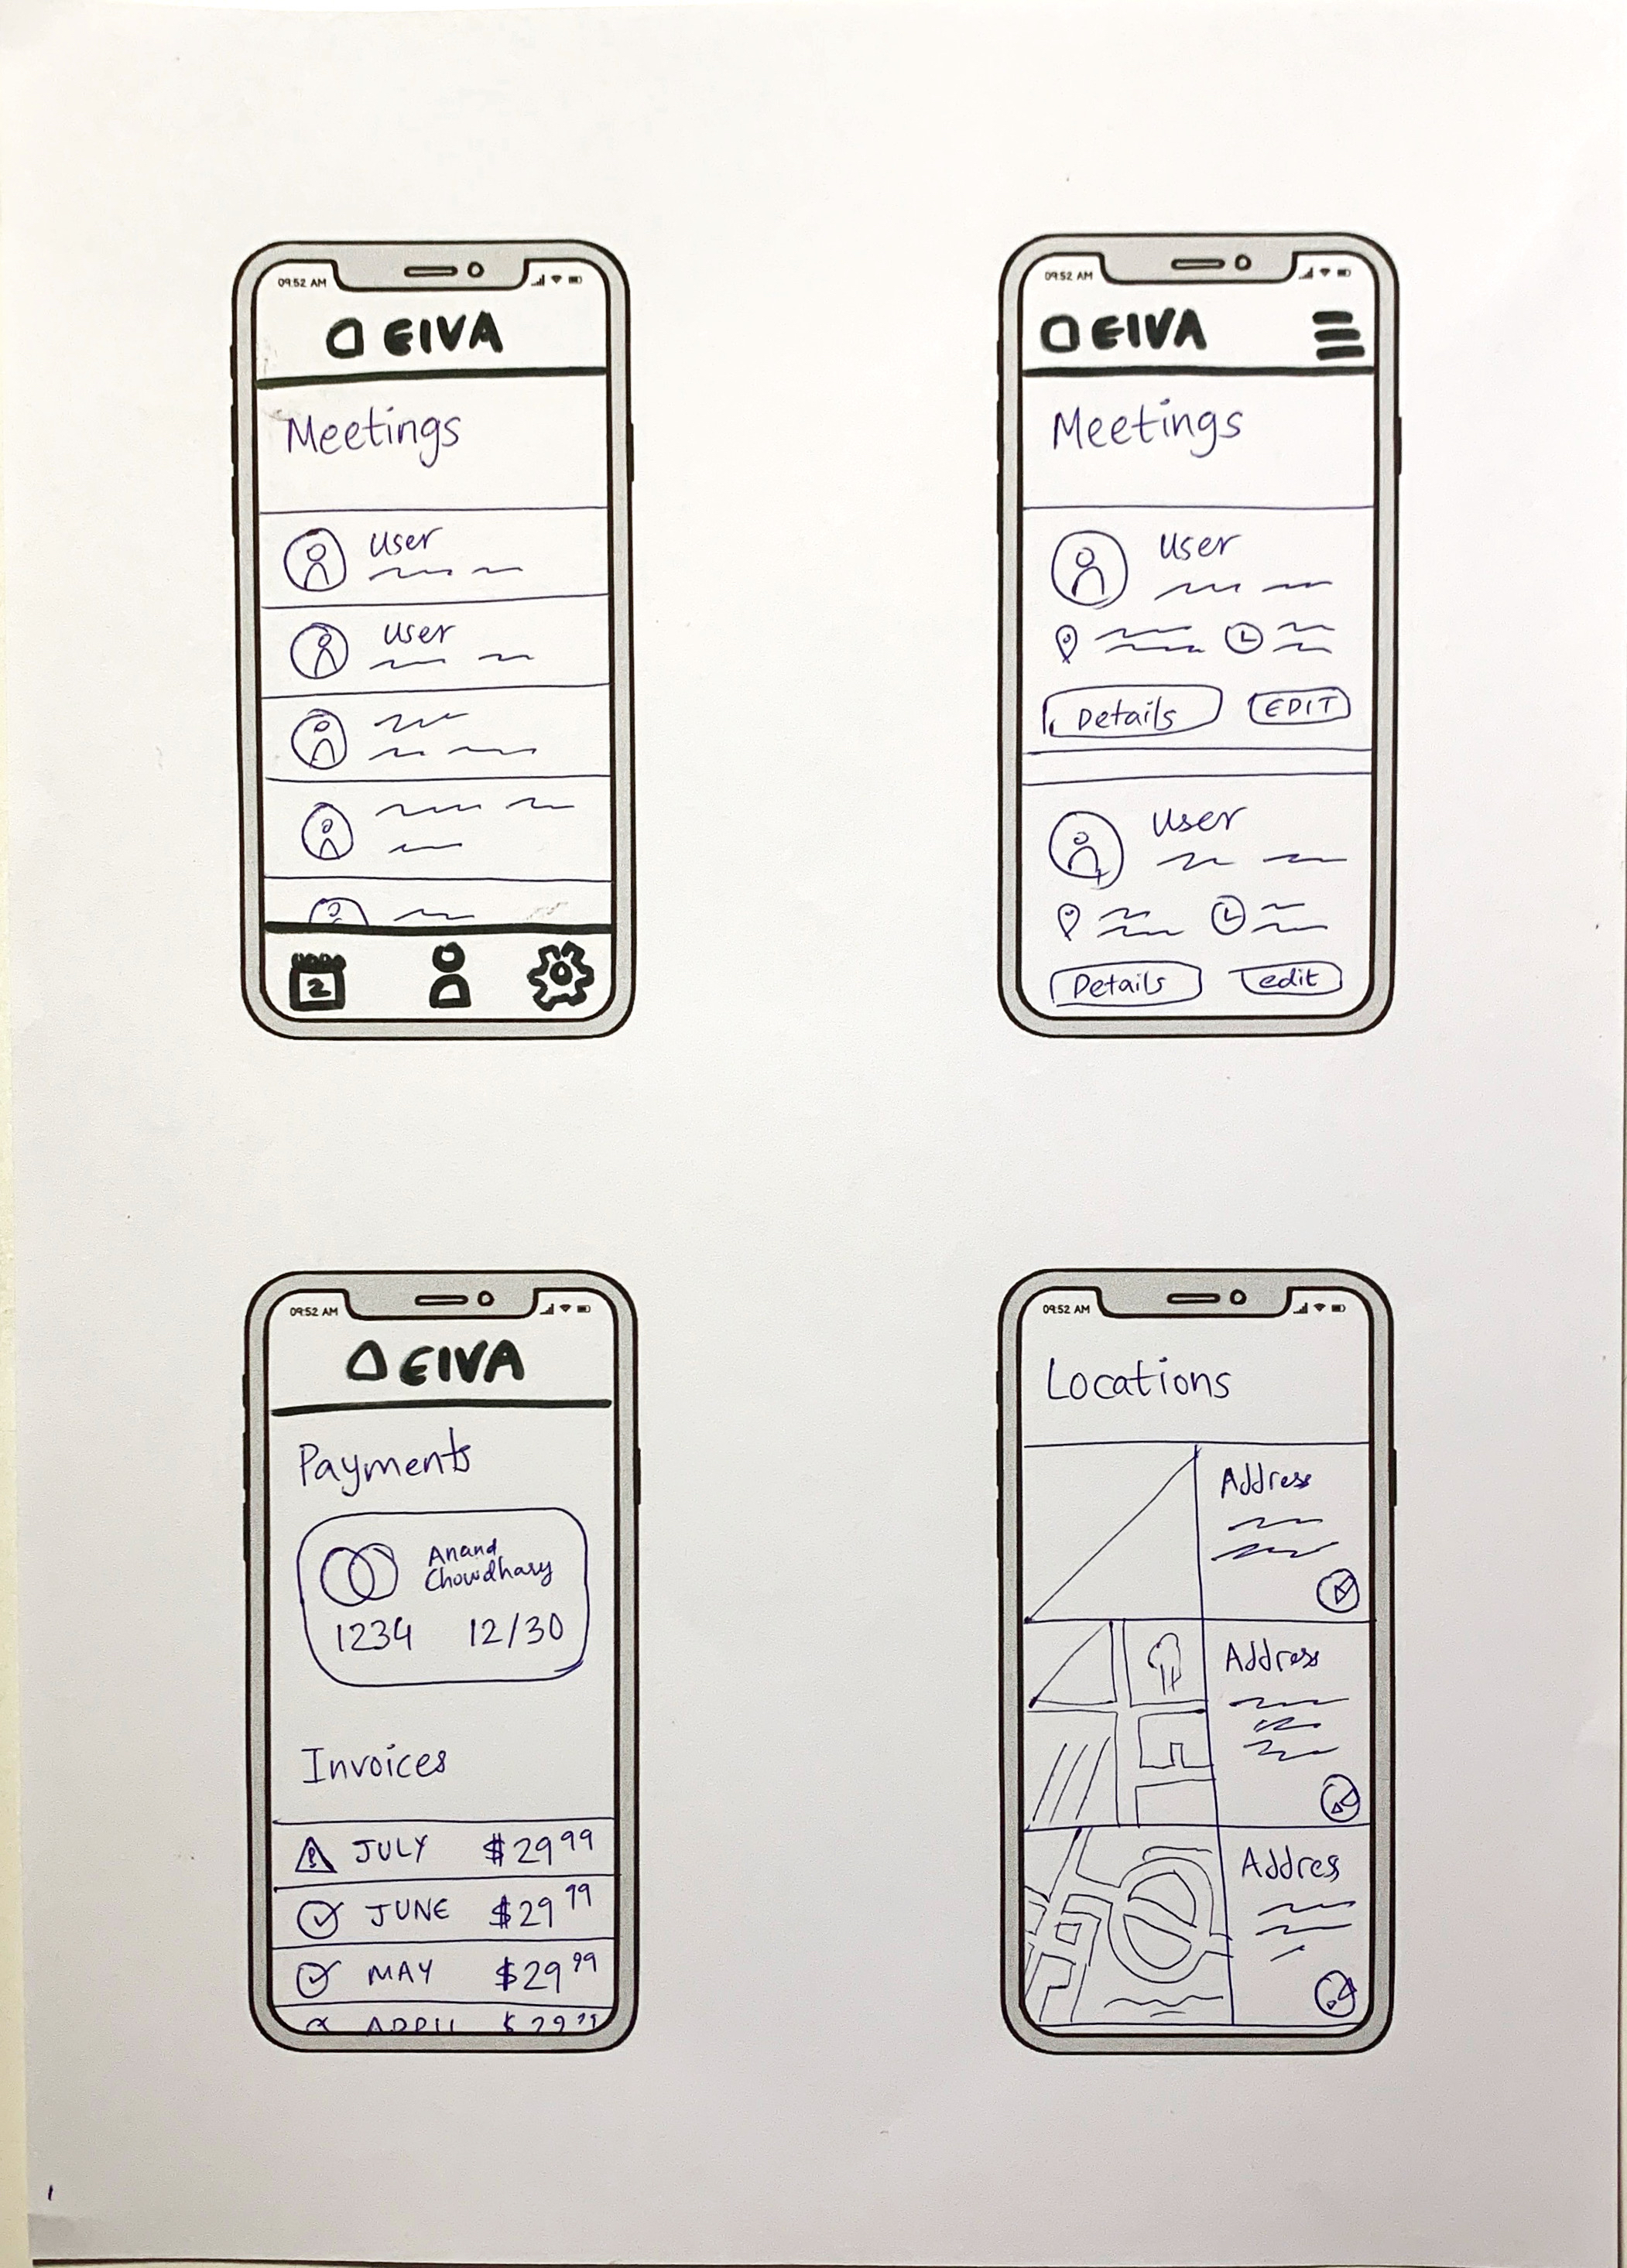
\includegraphics[width=1\linewidth]{drawing-phone-4.jpg}
	\end{minipage}
	\caption{Mobile Wireframes on Paper}
\end{figure}

...text...

\begin{figure}
  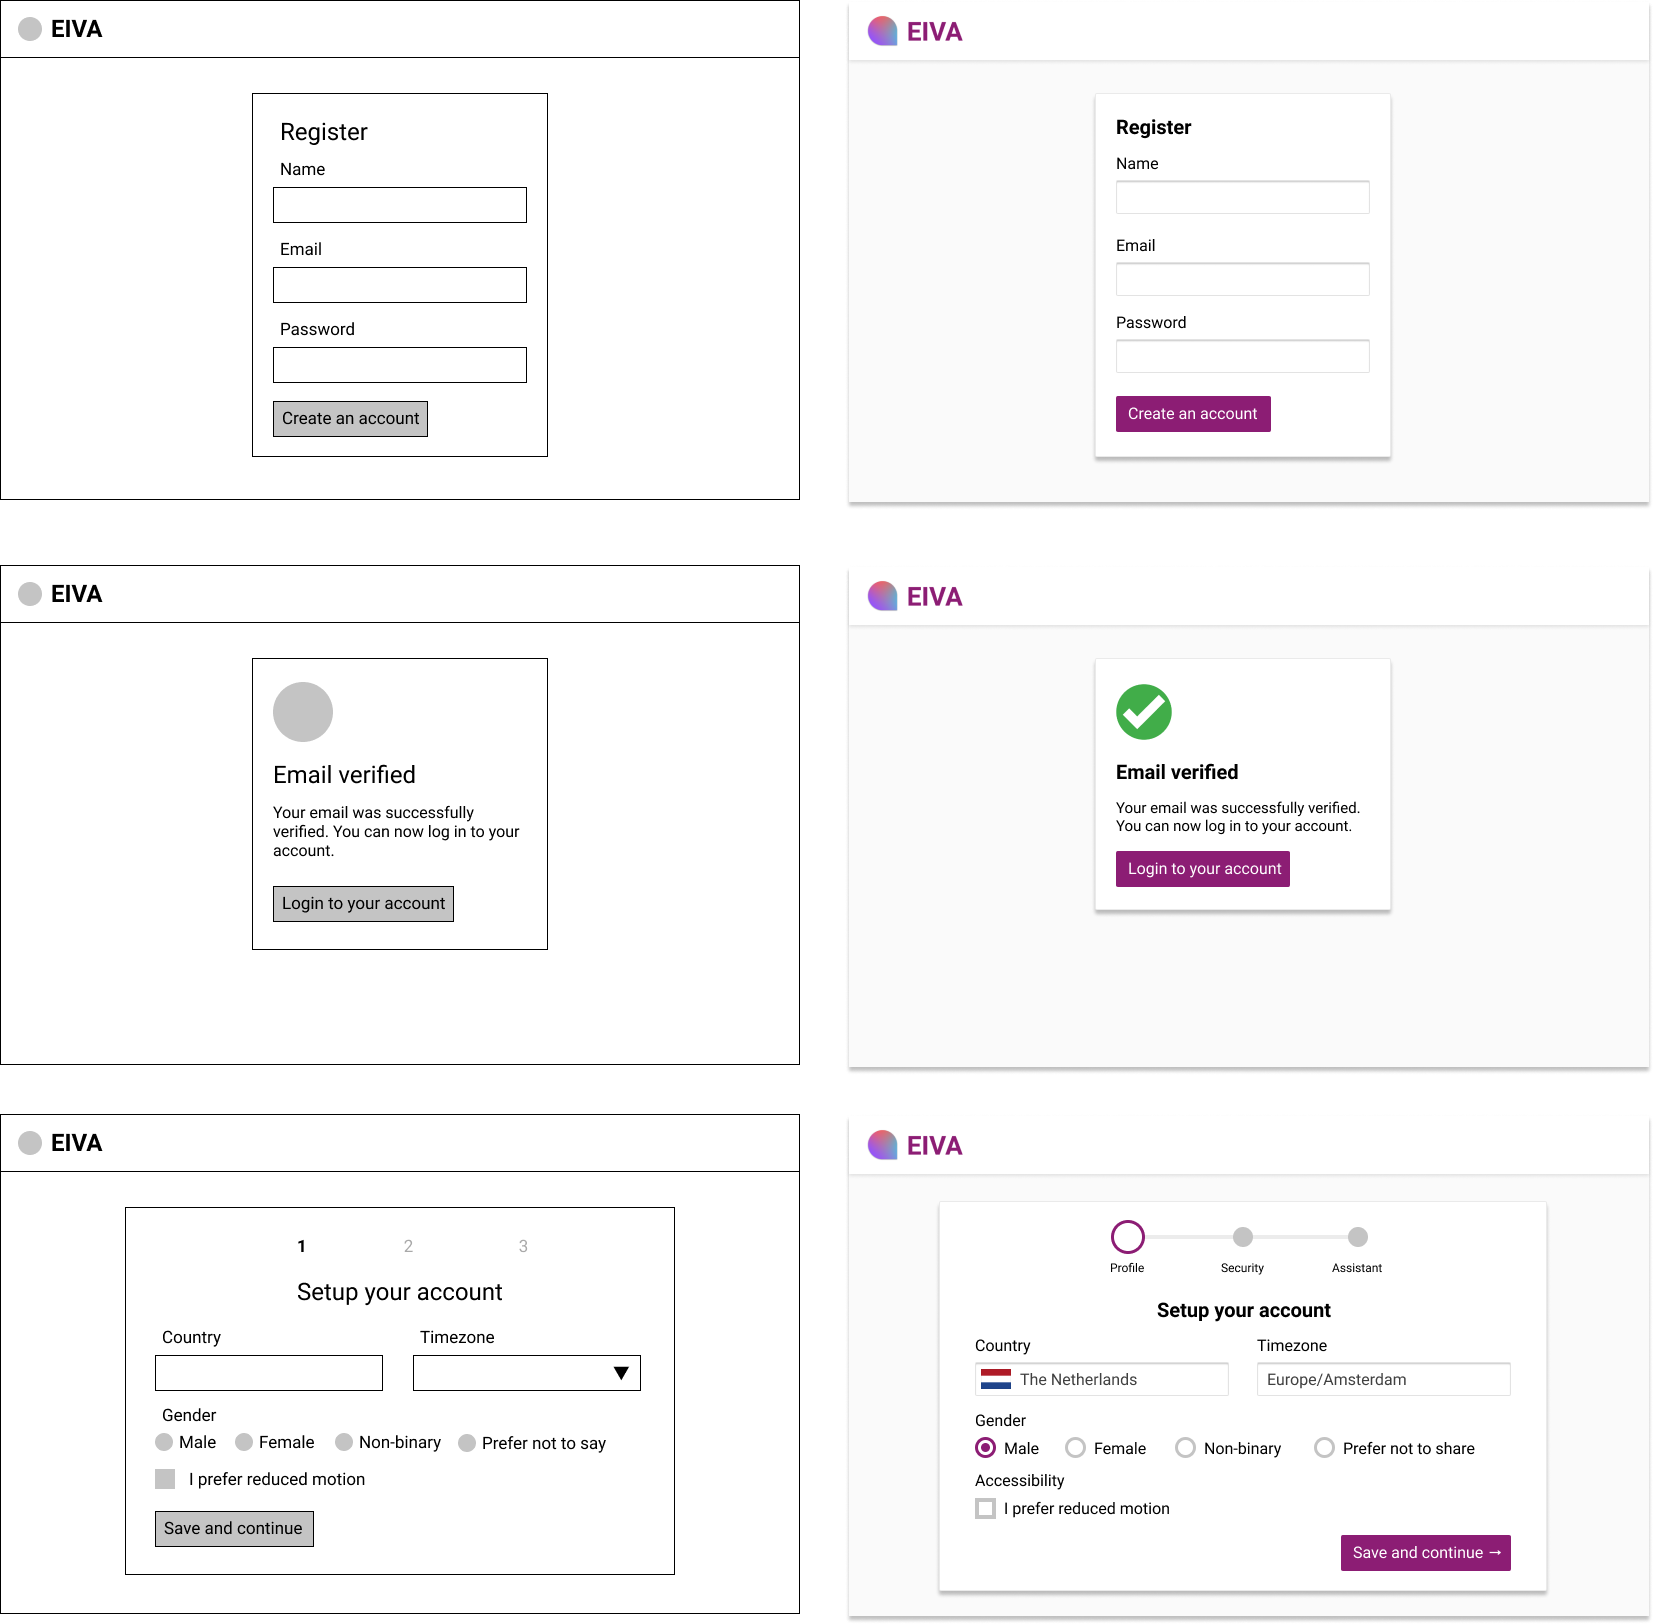
\includegraphics[width=\textwidth]{mockup-1.png}
  \caption{Comparison of low- and high-fidelity mockups}
\end{figure}

...text...

\newpage

\section{Specification}

This section will discuss the specifics on how the EIVA will be built.

\subsection{Tasks required in scheduling by an EIVA}

Since the majority of currently available scheduling tools are not assistant-based, most users prefer to use email for scheduling rather than currently available specialized software. A survey of workers in the field of information management found that over 80\% of the respondents use email for scheduling and organization \cite{ducheneaut_e-mail_2001}.

The process of scheduling online appointments is non-trivial and requires several rounds of communication, coordination, and negotiation.

\subsubsection{Understanding natural language over email}

Communication with devices using natural language is commonplace for many people today, especially with the advent of affordable smart voice assistants, such as Alexa, available on Amazon Echo; and Google Assistant, available on Google Home \cite{de_barcelos_silva_intelligent_2020}. Their interface, which translates a human's intention into a device's control commands using speech recognition and natural language interpretation, is known as a Natural Language Interface (NLI). The dialogue-style nature of the interactions between the user and the device and their ability to preserve context across different queries are benefits of using NLIs over other user interfaces \cite{kiseleva_predicting_2016}.

Personification of the scheduling process using natural language has the additional benefit of increased likeliness of error forgiveness by end users. In a study, over 80\% of the participants who encountered errors in NLIs understanding them said that either their attitude was unaffected or the users themselves ``must have typed in something wrong" \cite{kelley_iterative_1984}. Furthermore, NLIs allow people to use their existing calendaring tools and idiosyncrasies by adopting email as the user interface and natural language conversations as the interaction mode. For example, a message such as ``Please schedule an appointment with Florian for next week" should be enough for the EIVA to take over the remainder of the process.

\subsubsection{Parameter recommendations}

Recommendation systems are frequently used in several industries to help users make better decisions. Examples of collaborative recommender systems include product recommendations on e-commerce website Amazon \cite{linden_amazoncom_2003} and TV series recommendations on the streaming provider Netflix \cite{gomez-uribe_netflix_2016}. Modern systems may use various machine learning techniques like artificial neural networks combined with feature extraction methods to find the ideal recommendation \cite{adomavicius_toward_2005}.

Scheduling a single appointment requires agreement on several parameters, such as date, time, duration, and location of meeting. Recommending a set of these parameters must be based on the user's predetermined preferences, such as the hours they prefer for scheduling calls. However, the ideal implementation of such a recommendation system may take a multidimensional approach that uses additional contextual information \cite{adomavicius_incorporating_2005}. For example, contextual information may include the user's location to account for the travel time to a recommended meeting's location; or, for international calls, it may include the guest's timezone based on their IP address.

\subsubsection{Negotiation}

Since not all guests may be available at the initially proposed time, the next major task required by the EIVA is negotiation. The negotiation mechanism allows it to be flexible about constraints imposed by the preferences of other users. Zunino and Campo (2009) note that the negotiation mechanism ``starts when two [users] do not agree on some parameter of a meeting," such as the date, time, or location of the meeting \cite{zunino_chronos_2009}. Then, the guest may propose a new set of parameters for the meeting, for example by modifying its time. The EIVA will evaluate whether the proposal is convenient or not by comparing the ``likeliness of reaching a consensus using the previous meeting parameters with the proposed parameters." In this step, it can also make a judgement call by choosing to ignore part of the user's preferred parameters in order to agree with the guests. This back-and-forth negotiation process needs to occur asynchronously, ``sometimes requiring several days for the parties to reach consensus" \cite{cranshaw_calendarhelp_2017}.

\subsubsection{Renegotiation and confirmation invitations}

In the dynamic environment that is the modern workplace, changing appointment parameters is commonplace. A study found that 66\% of all scheduled meetings by a CEO underwent a parameter change \cite{dennis_how_2018}. Inevitably, once a meeting is scheduled, it requires ``continuous maintenance, as new events often prompt meeting updates and reschedules" \cite{cranshaw_calendarhelp_2017}. To finalize the meeting parameters, the EIVA should take into account the parameter preferences of both the user and all guests.

To make sure that all guests have the most recent parameters, confirmations and reminders may be sent by the EIVA. However, not all users use the same calendaring software, with some professionals using no digital calendar at all. Kincaid (1985) reported that approximately one half of all meetings scheduled by professionals were with users using a different calendaring system than their own \cite{kincaid_electronic_1985}. Therefore, the EIVA will be required to send these emails using industry standards supported by most software. The primary standard to store and exchange calendaring and scheduling information is the Internet Calendaring and Scheduling Core Object Specification (iCalendar) \cite{desruisseaux_internet_2009}.

\subsection{OK}

\newpage

\section{Realization}

\subsection{Appointment Scheduling}

\begin{wrapfigure}{l}{0.5\textwidth}\centering
	
\includegraphics[scale=0.4]{schedule-process.png}
	\caption{Appointment setup process}
\end{wrapfigure}

\subsection{Product Development}

A simplified version of the Software Development Life Cycle and the New Product Development Process were adopted for this project, with the following steps:

\begin{enumerate}
	\item Idea
	\item Research
	\item Development
	\item External testing
	\item Analysis
\end{enumerate}

The first step (Idea) builds on top of the ideation phase with methodological exploration of the idea and specifying the required feature as a module. In the second step (Research), the technical literature research present in ``State of the Art" is studied to architect the module's technology. In the third step (Development), the idea is materialized by writing code and testing the module by writing unit tests and conducting end-to-end tests with the platform. In the fourth step (External testing), a test is conducted with the client or research participants. In the last step (Analysis), the feedback from the test is evaluated for the next cycle.

\begin{figure}
	\centering
	\begin{minipage}{.4\textwidth}
		\centering
		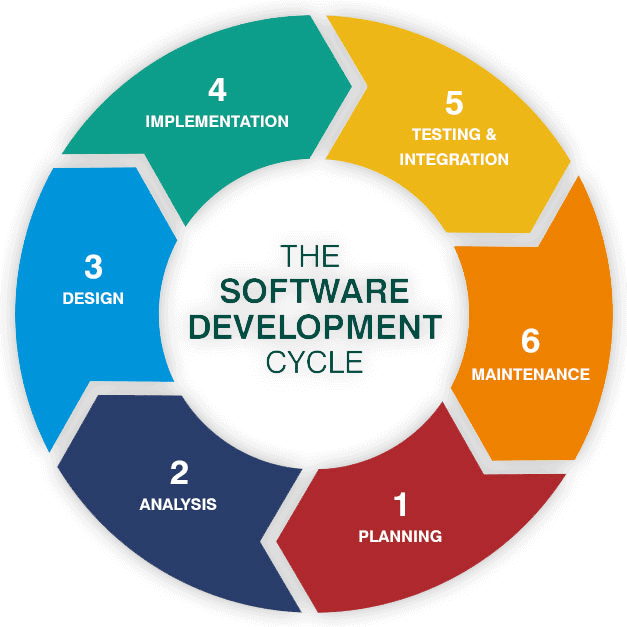
\includegraphics[height=.75\linewidth]{software-cycle.png}
		\captionof{figure}{The Software Development Cycle \cite{vlasova_7_nodate}}
		\label{fig:test1}
	\end{minipage}%
	\hspace{.5cm}
	\begin{minipage}{.4\textwidth}
		\centering
		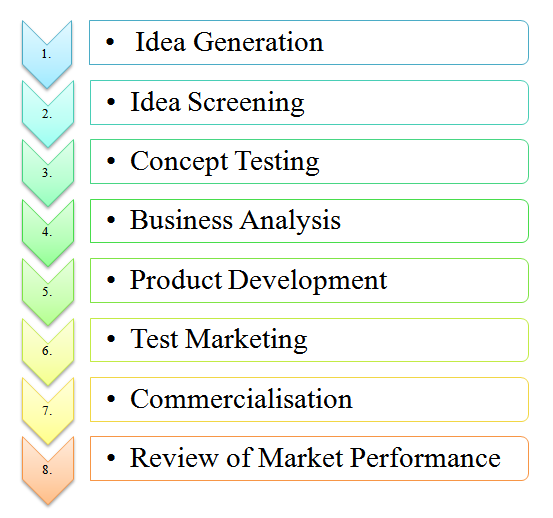
\includegraphics[height=.75\linewidth]{product-cycle.png}
		\captionof{figure}{The New Product Development Process \cite{akrani_stages_nodate}}
		\label{fig:test2}
	\end{minipage}
\end{figure}

\subsubsection{Cycle 1}

The first cycle was internal with both the initial development and several refactors. This was the only cycle that did not undergo an external test.

\paragraph{Assistant Email Address}

One of the specification conditions was to ensure unique email addresses for each organization using the assistant service, because teams may have similar names of assistants. For example, the default name of the assistant, ``Ara Isaacson", may generate the email address ``ara@araassistant.com", which does not share any information about who the assistant works for. Since unique email addresses for each team is mandatory, the team's slug was incorporated in the address, i.e., ``username@araassistant.com", for example ``florian@araassistant.com". This has two advantages: firstly, it tells the guests receiving emails from the assistant who the true host is; and secondly, the email receiving architecture can relate the unique email address to the owner's details.

However, in the first cycle itself, the assistant's default email was changed from ``username@domain" to ``meet-username@domain" where ``username" is the organization slug and the domain is the assistant's service domain. This was done to prevent confusion based on the email address; for example, ``florian@araassistant.com" may be mistaken as the email address of Florian himself (the user), whereas ``meet-florian@araassistant.com" implies that the email address is of the assistant, using which you can schedule an appointment with Florian.

\subsubsection{Cycle 2}

Privacy features, privacy onboarding

\subsubsection{Cycle 3}

Support for non-Google Calendar with iCal

\subsubsection{Cycle 4}

NLP in multiple languages rather than translation \thesubsubsection

\subsubsection{Cycle 5}

Slack, email from Florian

\subsubsection{Cycle 6}

External feedback from Rohit, Maurits, Alex

\subsection{Open Source Development}

Although the preceding project Ara was licensed under the open source permissive MIT license, EIVA's source code is made available under the Server Side Public License. This license makes sure that any further implementations or paid services built around EIVA also have their source code made public, and helps the future business use case of EIVA.

However, several open source projects were built in order to support key EIVA features, which were all licensed under the MIT license. This encourages wide community adoption and contributes back to the open source ecosystem, as MIT is the most popular open source license and allows commercial usage of open source projects.

For example, the open source project ``calendar-link" was built in order to generate event links to popular calendar services like Google Calendar, Microsoft Outlook, and Yahoo! Calendar. This project is now used by many others, receiving over 1,000 downloads every week and contributed to by 5 additional developers. Developers can use the package to programmatically generate that users can click on to add a specific event to their calendar, with an easy-to-use API:

...

Similarly, another project ``calendar-slots" was released to help find available slots in a user's calendar. This package can save development times when recommending appointment slots by listing a user's calendars, fetching all events in a given timeframe, removing slots with conflicts with scheduled events, and recommending a fixed number of slots to the end user:

...

It is also highly configurable, with support for settings such as timezone preference, daily scheduling hours, and custom filter options:

...

Both projects are written in TypeScript and available on the Git hosting service GitHub and JavaScript package registry NPM.

\subsection{Software Tests}

\subsubsection{Unit Tests}

Unit tests are used \cite{tosun_effectiveness_2018}.

dates.spec.ts

\subsubsection{Continuous Integration}

CI is used \cite{li_extensive_2020}.

\paragraph{End-to-end Tests} ...

\subsection{Deployment}

AWS is used \cite{shokeen_deploying_2019}. AWS is secure \cite{narula_cloud_2015}. Oswald Labs Accelerator credits \cite{noauthor_oswald_nodate}.

Info about deployment, server, etc. There is a script ``update.sh" with the following lines.

...


Each line does this respectively… in the future, load balancers, etc.

\subsubsection{Server Monitoring}

\paragraph{Uptime Monitoring}

Although measures have been taken to make sure EIVA services don't go down, such as installing Cloudflare' Always Online which serves a static version of a webpage if it is not available from the origin server \cite{noauthor_keep_nodate}, there is sometimes nothing one can do to prevent a website from going down. ``Traffic spikes, malware attacks, data center problems, etc." can cause server downtime \cite{noauthor_what_2018}.

To monitor the uptime of the services and get real-time notifications in case of downtime, \emph{Uptime Robot} is installed \cite{noauthor_about_nodate}. In intervals of 5 minutes, Uptime Robot makes network requests to the frontend and backend URLs, logs the response time (Figure), and sends an email and Slack notification in case any URL is unavailable.

Over the course of testing weeks, no downtime was recorded for the backend, but the frontend was unavailable twice for a period of 2 minutes and 57 seconds and 2 minutes and 44 seconds on June 7 and June 9 2020 respectively. This was due of a Netlify deploying error because of renamed respositories. Both times, this error was immediately fixed because of the real-time notifications feature, and resulted in a $>$ 99.9\% overall uptime.

\begin{figure}
	\centering
	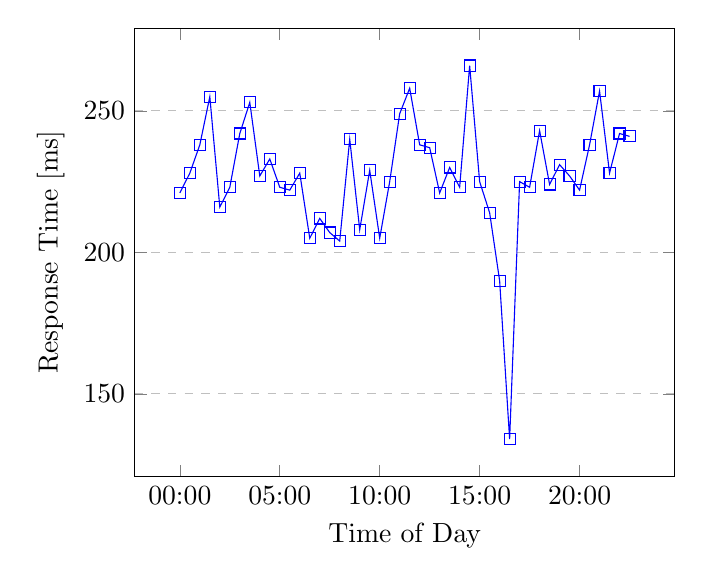
\begin{tikzpicture}
		\begin{axis}[
				xlabel={Time of Day},
				ylabel={Response Time [ms]},
				legend pos=north west,
				ymajorgrids=true,
				grid style=dashed,
				xticklabels={0,00:00,05:00,10:00,15:00,20:00}
			]
			
			\addplot[
				color=blue,
				mark=square,
			]
			coordinates {
				(0, 221)(1, 228)(2, 238)(3, 255)(4, 216)(5, 223)(6, 242)(7, 253)(8, 227)(9, 233)(10, 223)(11, 222)(12, 228)(13, 205)(14, 212)(15, 207)(16, 204)(17, 240)(18, 208)(19, 229)(20, 205)(21, 225)(22, 249)(23, 258)(24, 238)(25, 237)(26, 221)(27, 230)(28, 223)(29, 266)(30, 225)(31, 214)(32, 190)(33, 134)(34, 225)(35, 223)(36, 243)(37, 224)(38, 231)(39, 227)(40, 222)(41, 238)(42, 257)(43, 228)(44, 242)(45, 241)
			};
			
		\end{axis}
	\end{tikzpicture}
	\caption{24-Hour Response Time of the EIVA website}
\end{figure}

\paragraph{Resource Monitoring}

\emph{Netdata} is used \cite{noauthor_netdata_nodate}. NetData is open source \cite{noauthor_netdata/netdata_2020}.

\paragraph{Event Tracking}

\emph{ElasticSearch} is used \cite{noauthor_elastic_nodate}. ElasticSearch is open source \cite{noauthor_elastic/elasticsearch_2020}. Open Distro for ElasticSearch is used for increased security, including data encryption at rest and Kibana authentication \cite{noauthor_open_nodate}.

As an example, Figure 6 shows that number of event tracked (pageviews and clicks) during the first ten days of June 2020. The average number of events tracked per day was 1,062.4.

\subsubsection{Catching Errors}

To catch errors in production, \emph{Sentry} is deployed in both the frontend and backend applications. Sentry is an open source error tracking system \cite{noauthor_sentry_nodate} that automatically reports errors as soon as they occur. ``In addition to sending developers alerts, Sentry also gives them context for potential root cause analysis to help them identify the source of the error" \cite{noauthor_sentry_nodate-1}.

Although the backend project collects server logs, they are frequently intentional debugging information. Logging provides a trail of events, but Sentry only focuses on exceptions, i.e., catching application crashes or HTTP request errors. Furthermore, Sentry helps list a trail of usage events like mouse clicks and network requests to discover the context of an error \cite{noauthor_sentry_nodate-2}.

Licensed under Apache 2, Sentry is open source but offers a hosted service with a generous free plan, which is used for this project. The @sentry/browser package is used to track errors originating in client-side web applications running in browsers, and @sentry/node is used for the Node.js package.

Over the course of testing weeks, 3 errors were tracked for the frontend project, but no errors were found in the backend project.

\subsection{User Experience Research}

After building and deploying a functional virtual agent and its companion web application, a user experience research is conducted with participants with diverse backgrounds. The user experience research is completely virtual and divided in three parts:

\begin{enumerate}
	\item Introductory Survey
	\item Product Usage
	\item User Experience Evaluation
\end{enumerate}

The questions are specifically written in a first-person form, as the assistant also interacts, and additional information has been included when asking for potentially personal details. Options in multiple choice questions are randomized to eliminate order bias.

\subsubsection{Introductory Survey}

After reading the Information Brochure (Appendix 1.1) signing the Consent Form (Appendix 1.2), participants answer 16 questions about their prior experience with scheduling appointments, email usage, and personal assistants. This information helps with understanding how users currently set appointments, and with setting the default values for settings (Section 6.2).

Appendix 1.3 lists all the options for each question. The Introductory Survey is divided into two parts; the first part is focuses on scheduling preferences and email usage:

\begin{enumerate}
	\item Which type of profession best describes you? This helps us relate scheduling experience with types of work.
	\item Say you had to schedule an appointment with a colleague (if you're a professional) or a professor (if you're a student). How would you do it?
	\item How frequently do you check your email, on average, on working days?
	\item What languages do you send emails in? Enter as many as you like.
	\item Do you have email notifications enabled on your phone?
	\item What service do you use for your primary email account?
	\item What do you use email for? Select as many as you like.
	\item What calendar service do you use, if any? Select as many as you like.
\end{enumerate}

The second part asks participants about using personal assistants for scheduling:

\begin{enumerate}[resume]
	\item If you had a personal assistant, would you ask them to schedule your appointments for you?
	\item Imagine that you had an AI-powered, virtual personal assistant who could set up appointments for you by finding available times in your calendar and sending emails on your behalf. Would you use this service?
	\item Say that you ask your virtual assistant to schedule an appointment with someone. For the recipient, this email would be indistinguishable from an email sent by a human assistant. Should the virtual assistant inform the recipient that it is not a human, but an AI-powered virtual assistant?
	\item Should recipients be able to unsubscribe from your assistant's emails, i.e., "opt out" of talking to an AI, and choose to only communicate with you instead?
	\item Would you like to know whether or not someone has seen an email sent by the assistant?
	\item If you have enabled email tracking, should end users know that a read receipt has been shared, i.e., a notice at the end of the email, "The sender has been notified that you've opened this email"?
	\item Apart from scheduling appointments, what else would you like your virtual assistant to do, over email?
\end{enumerate}

\subsubsection{Product Usage}

After finishing the Introductory Survey, participants start using the assistant service with the help of virtual guides consisting of several screenshots, an onboarding wizard, and an introductory tour.

The participants open the web application on \url{https://myeiva.com} and create an account. After creating their account, the verify their email and log into their accounts. They then complete the onboarding flow, setting up basic information such as their name, timezone, gender, security preferences, and name of their assistant.

Then, they follow an introductory tour which helps them customize their assistant's settings, add additional meeting locations, etc., before sending an email to their assistants. After sending an email to schedule an appointments, participants go back to the survey for the UX evaluation.

\subsubsection{User Experience Evaluation}

In the last part, participants answer questions about the experience of both the assistant and the web application in the form of another survey:

\begin{enumerate}
	\item What comes to mind when you think about EIVA (how would you describe it to a friend)?
	\item On a scale from 1 to 5, review the following about the web app. 1 is the worst and 5 is the best:
	      \begin{enumerate}
	      	\item Overall experience of the web app (not the assistant)
	      	\item Design of the web app
	      	\item Functionality of the web app
	      	\item Ease of use of the web app
	      	\item Privacy features available in the web app
	      	\item Overall experience of the onboarding flow
	      	\item Overall experience of the introductory tour
	      \end{enumerate}
	\item On a scale from 1 to 5, review the following about the assistant. 1 is the worst and 5 is the best:
	      \begin{enumerate}
	      	\item Overall experience of the assistant over email
	      	\item Customizability of the assistant
	      	\item Flexibility in understanding natural language
	      	\item How human-like does the assistant sound over email? 1 is not human-like at all and 5 is indistinguishable from a human.
	      	\item How much do you trust the assistant to not make mistakes? 1 is the least trust and 5 is the most.
	      	\item How accurate, practical, and logical were the time recommendations made by the assistant?
	      \end{enumerate}
	\item How many emails did you sent with the assistant in CC?
	\item Did the assistant understand your email(s) correctly?
	\item Did the assistant respond to your email in a reasonable amount of time?
	\item Did the assistant recommend the correct location for the appointment?
	\item Did the assistant meet your expectations in terms of scheduling an appointment?
	\item Which of these features of the web app did you use?
	\item If you were the recipient of an email from EIVA, would you be able to tell whether it's an email from an AI or human assistant, if you didn't know?
	\item If we launch EIVA as a service where users can get their own assistants, will you use it?
	\item Based on the amount of time EIVA saves when setting appointments, how much would you be willing to pay for such a service?
	\item Did you find anything frustrating that you wish was easier or different?
	\item Is there anything that you wish the assistant could do, in terms of scheduling, that it doesn't currently?
	\item What do you like the most about EIVA?
	\item What do you like the least about EIVA?
	\item Do you have any additional feedback, suggestions, or comments?
\end{enumerate}

\newpage

\section{Evaluation}

This section will discuss the results of UX research, what features people like, their privacy preferences, ease of use, analytics from the app, etc.

10 users from 6 countries and territories participated in this research: Bonaire, India, Iran, the Netherlands, Poland, and the United States. However, Table 11 in Section 7.2 highlights that users from several other countries also visited the app, but didn't participate in the research.

\subsection{Introductory Survey}

A diverse group of users participated in the survey, both working professionals and students. 4 out of 10 respondents were employed full-time by a company or organization, another 4 were students, and 2 out of 10 were freelancers or self-employed individuals (Table 1).

\begin{table}[!htb]
	\begin{minipage}{.5\linewidth}
		\caption{Professions of Participants}
		\centering
		\begin{tabular}{lr}
			\hline
			\textbf{Profession} & \textbf{Percentage} \\
			\hline
			Employed            & 40\%                \\
			Student             & 40\%                \\
			Self-employed       & 20\%                \\
			\hline
		\end{tabular}
	\end{minipage}%
	\hspace{.1cm}
	\begin{minipage}{.5\linewidth}
		\centering
		\caption{Preferred Modes of Scheduling}
		\begin{tabular}{lr}
			\hline
			\textbf{Mode}        & \textbf{Percentage} \\
			\hline
			Send an email        & 70\%                \\
			Work chat message    & 40\%                \\
			Consumer chat        & 40\%                \\
			Phone call           & 30\%                \\
			Go to office or desk & 10\%                \\
			\hline
		\end{tabular}
	\end{minipage} 
\end{table}

In Table 2, `Work chat' refers to instant messaging services like Slack and Microsoft Teams whereas `Consumer chat' refers to services like WhatsApp and Facebook Messenger, and participants could choose multiple options. The results show a preference for emails, as noted in State of the Art (Section 2). Apart from email, chat services are popular with users too, whereas physically reaching out is the least often used.

\subsubsection{Email and Calendar Usage}

To identity whether email is the ideal use case, participants were asked about their frequency of checking their email (Table 4) and sending emails (Table 3).

Most participants (80\%) check their email multiple times per day, whereas only 1 in 10 users check their email at least once per day or week. 5 out of 10 participants send one or more emails every day, where 4 in 10 and 1 in 10 participants send new emails every day or week respectively.

\begin{table}[!htb]
	\begin{minipage}{.5\linewidth}
		\caption{Frequency of Emails Sent}
		\centering
		\begin{tabular}{lr}
			\hline
			\textbf{Number of Emails} & \textbf{Percentage} \\
			\hline
			One or more per day       & 50\%                \\
			One every few days        & 40\%                \\
			One every few weeks       & 10\%                \\
			\hline
		\end{tabular}
	\end{minipage}%
	\hspace{.1cm}
	\begin{minipage}{.5\linewidth}
		\centering
		\caption{Frequency of Checking Email}
		\begin{tabular}{lr}
			\hline
			\textbf{Number of Times} & \textbf{Percentage} \\
			\hline
			Multiple times per day   & 80\%                \\
			At least once per day    & 10\%                \\
			At least once per week   & 10\%                \\
			\hline
		\end{tabular}
	\end{minipage} 
\end{table}

Since EIVA supports both English and Dutch, participants were asked their preferred languages for email communication. All participants selected English, 3 in 10 participants also chose Dutch, and 1 participant also selected Polish.

For better integration with large email providers, participants were also asked about their primary email service provider. Half of all participants use Google's Gmail or G Suite, 2 in 10 use a Microsoft service (like Hotmail or Live), and 1 in 10 use each of Yahoo!, custom hosted SMTP, or others.

Furthermore, they were asked whether they have email notifications enabled on their smartphones, to which all participants responded in the affirmative.

\begin{table}[!htb]
	\begin{minipage}{.5\linewidth}
		\caption{Email Languages}
		\centering
		\begin{tabular}{lr}
			\hline
			\textbf{Language} & \textbf{Percentage} \\
			\hline
			English           & 100\%               \\
			Dutch             & 30\%                \\
			Polish            & 10\%                \\
			\hline
		\end{tabular}
	\end{minipage}%
	\hspace{.1cm}
	\begin{minipage}{.5\linewidth}
		\centering
		\caption{Email Service Providers}
		\begin{tabular}{lr}
			\hline
			\textbf{Service} & \textbf{Percentage} \\
			\hline
			Google           & 50\%                \\
			Microsoft        & 20\%                \\
			Yahoo!           & 10\%                \\
			SMTP             & 10\%                \\
			Other            & 10\%                \\
			\hline
		\end{tabular}
	\end{minipage} 
\end{table}

Apart from scheduling, there are also several other reasons to use email. Participants were asked \emph{What do you use email for?}, and all participants selected work-related communication. 7 in 10 also chose scheduling appointments, while 3 in 10 use email to connect with friends and family. 2 out of 10 participants use email for outbound marketing, whereas 1 in 10 also use it for customer support.

\begin{table}[!htb]
	\begin{minipage}{1\linewidth}
		\caption{Reasons for Sending Emails}
		\centering
		\begin{tabular}{lr}
			\hline
			\textbf{Reason}                         & \textbf{Percentage} \\
			\hline
			Other work-related communication        & 100\%               \\
			Scheduling appointments                 & 70\%                \\
			Connecting with friends and family      & 30\%                \\
			Sending marketing emails or newsletters & 20\%                \\
			Contacting customer support             & 10\%                \\
			\hline
		\end{tabular}
	\end{minipage}%
\end{table}

Although EIVA connects with any calendar application that follows the iCalendar standard, which all major services do, it also directly integrates with Google Calendar. This was chosen with the hypothesis that it's the most popular calendar service, which was proved to be true based on the participants' responses. Half of all participants selected Google Calendar as their primary calendar service, 4 out of 10 participants use Microsoft Outlook, and another 20\% each use Apple Calendar or no calendar. Lastly, 1 in 10 respondents use a custom, self-hosted calendar.

\begin{table}[!htb]
	\begin{minipage}{1\linewidth}
		\caption{Primary Calendar Services}
		\centering
		\begin{tabular}{lr}
			\hline
			\textbf{Reason}                   & \textbf{Percentage} \\
			\hline
			Google Calendar                   & 50\%                \\
			Microsoft Outlook                 & 40\%                \\
			Apple Calendar                    & 20\%                \\
			\emph{I don't use a calendar app} & 20\%                \\
			Self-hosted calendar              & 10\%                \\
			\hline
		\end{tabular}
	\end{minipage}%
\end{table}

\subsubsection{Personal Assistant for Scheduling}

In the second part of the Introductory Survey, participants were asked hypotheticals about using an assistant for scheduling meetings. The results of the six polar questions (yes/no) are tabulated in Table 9.

\begin{table}[!htb]
	\begin{minipage}{1\linewidth}
		\caption{Responses to Polar Question}
		\centering
		\begin{tabular}{p{10cm}p{2cm}}
			\hline
			\textbf{Question}                                                                               & \textbf{Percentage of `Yes'} \\
			\hline
			If you had a personal assistant, would you ask them to schedule your appointments for you?      & 90\%                         \\
			Would you use the EIVA service?                                                                 & 80\%                         \\
			Should EIVA inform recipients that it is not human?                                             & 60\%                         \\
			Should recipients be able to unsubscribe from EIVA emails?                                      & 60\%                         \\
			Would you like to know whether someone has seen an email sent by EIVA?                          & 40\%                         \\
			If you have enabled email tracking, should recipients know that a read receipt has been shared? & 70\%                         \\
			\hline
		\end{tabular}
	\end{minipage}%
\end{table}

Currently, EIVA only sets appointments but the big picture goal of EIVA is to automate several other workflows, like automatically responding to emails or sending outbound marketing emails. Participants were also asked what other features they would like to see.

Table 10 summarizes the most-requested additional features that participants want EIVA to have. 9 out of 10 respondents requested reminders, 7 out 10 selected automatic frequent email responses, and 6 out of 10 selected email follow-ups to team members. 2 out of 10 participants requested sending marketing emails, and 1 out of 10 self-requested emails with their schedule for the day.

\begin{table}[!htb]
	\begin{minipage}{1\linewidth}
		\caption{Most Requested Additional Features}
		\centering
		\begin{tabular}{lr}
			\hline
			\textbf{Feature}                & \textbf{Percentage} \\
			\hline
			Reminders                       & 90\%                \\
			Auto-respond to frequent emails & 70\%                \\
			Send email follow-ups           & 60\%                \\
			Send marketing emails           & 20\%                \\
			Daily schedule summary email    & 10\%                \\
			\hline
		\end{tabular}
	\end{minipage}%
\end{table}

\subsection{Product Usage}

Although participants were allowed to use the webapp in May 2020 and June 2020, for data consistency, only data stored in ElasticSearch between June 1 and June 10 is analyzed. This ten-day period was that of heaviest participation, and therefore can serve as an approximate for the entire research period. In this period, a total of 1,536 pageviews and 10,772 API logs were collected.

\subsubsection{Web App Traffic Analysis}

This section analyzes the pageviews tracked during the ten-day period. As described in Section 6.5.3, a JavaScript snippet was used to send information about each pageview to the ElasticSearch engine via the API, and most data was computed on the client, such as parsing the user agent.

\paragraph{Location}

Users from four continents used the web application -- Europe, Asia, Africa, and North America. The approximate location of users is determined based on their IP address using Maxmind's GeoIP2. Figure 8 and Table 11 highlight the nine countries --- the Netherlands, India, Poland, Kenya, the United States, Finland, Indonesia, Germany, and France.

Furthermore, in the Netherlands, usage was observed in 7 out of 12 province, with the maximum usage coming from Flevoland, followered in order by Overijssel, Gelderland, Utrecht, South Holland, North Holland, and Friesland. Table 12 and Figure 10 show the usage distribution in Dutch provinces, and Figure 9 shows an overview of usage coming from the continent of Europe.

\begin{figure}
  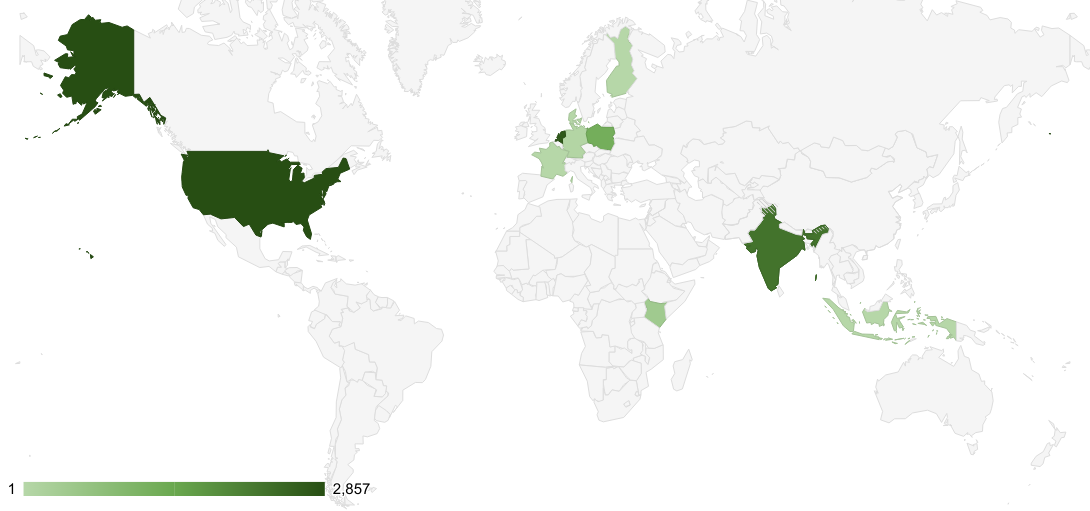
\includegraphics[width=\textwidth]{location-world.png}
  \caption{Usage by Country (Worldwide)}
\end{figure}

\begin{table}[!htb]
	\begin{minipage}{.5\linewidth}
		\caption{Usage by Country}
		\centering
		\begin{tabular}{lr}
			\hline
			\textbf{Country} & \textbf{Pageviews} \\
			\hline
			The Netherlands  & 584                \\
			India            & 514                \\
			Poland           & 237                \\
			Kenya            & 106                \\
			United States    & 83                 \\
			Finland          & 4                  \\
			Indonesia        & 4                  \\
			Germany          & 2                  \\
			France           & 2                  \\
			\hline
		\end{tabular}
	\end{minipage}%
	\hspace{.1cm}
	\begin{minipage}{.5\linewidth}
		\centering
		\centering
		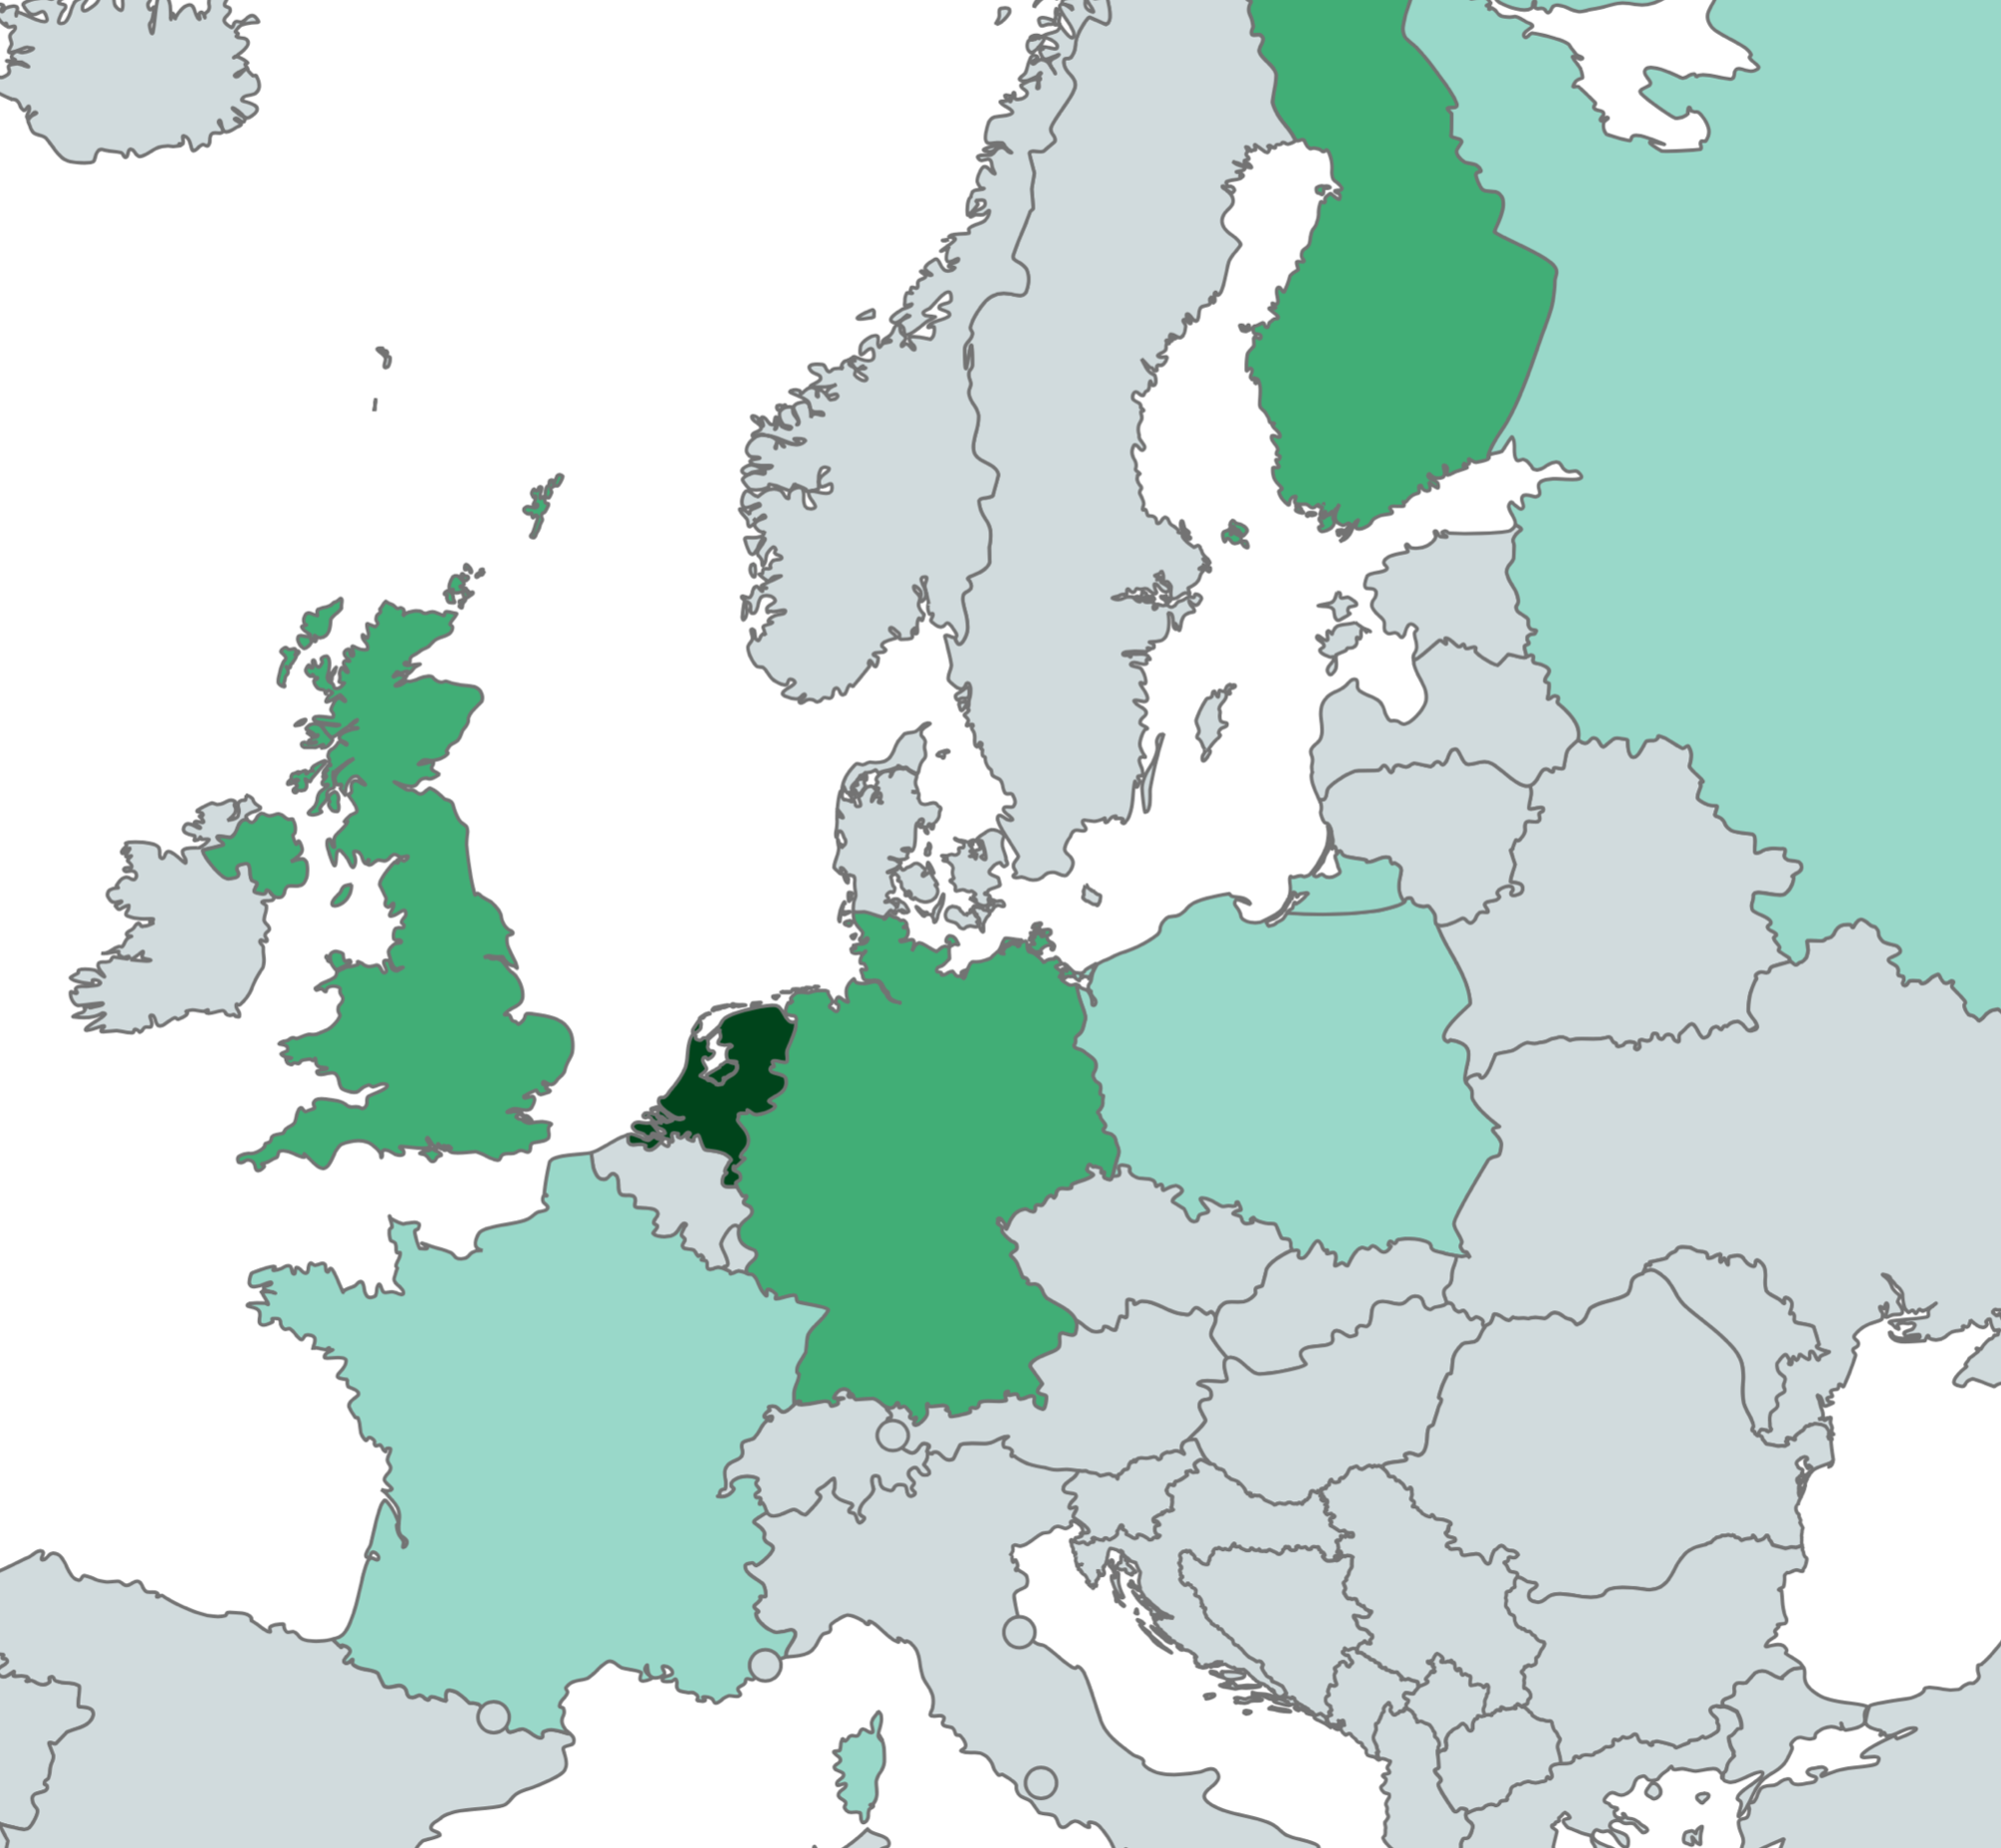
\includegraphics[width=1\linewidth]{location-europe.png}
		\captionof{figure}{Usage by Country (Europe)}
		\label{fig:test2}
	\end{minipage} 
\end{table}

\begin{table}[!htb]
	\begin{minipage}{.5\linewidth}
		\caption{Usage by Dutch Province}
		\centering
		\begin{tabular}{lr}
			\hline
			\textbf{Province} & \textbf{Pageviews} \\
			\hline
			Flevoland         & 348                \\
			Overijssel        & 116                \\
			Gelderland        & 39                 \\
			Utrecht           & 33                 \\
			South Holland     & 18                 \\
			North Holland     & 3                  \\
			Friesland         & 1                  \\
			\hline
		\end{tabular}
	\end{minipage}%
	\hspace{.1cm}
	\begin{minipage}{.5\linewidth}
		\centering
		\centering
		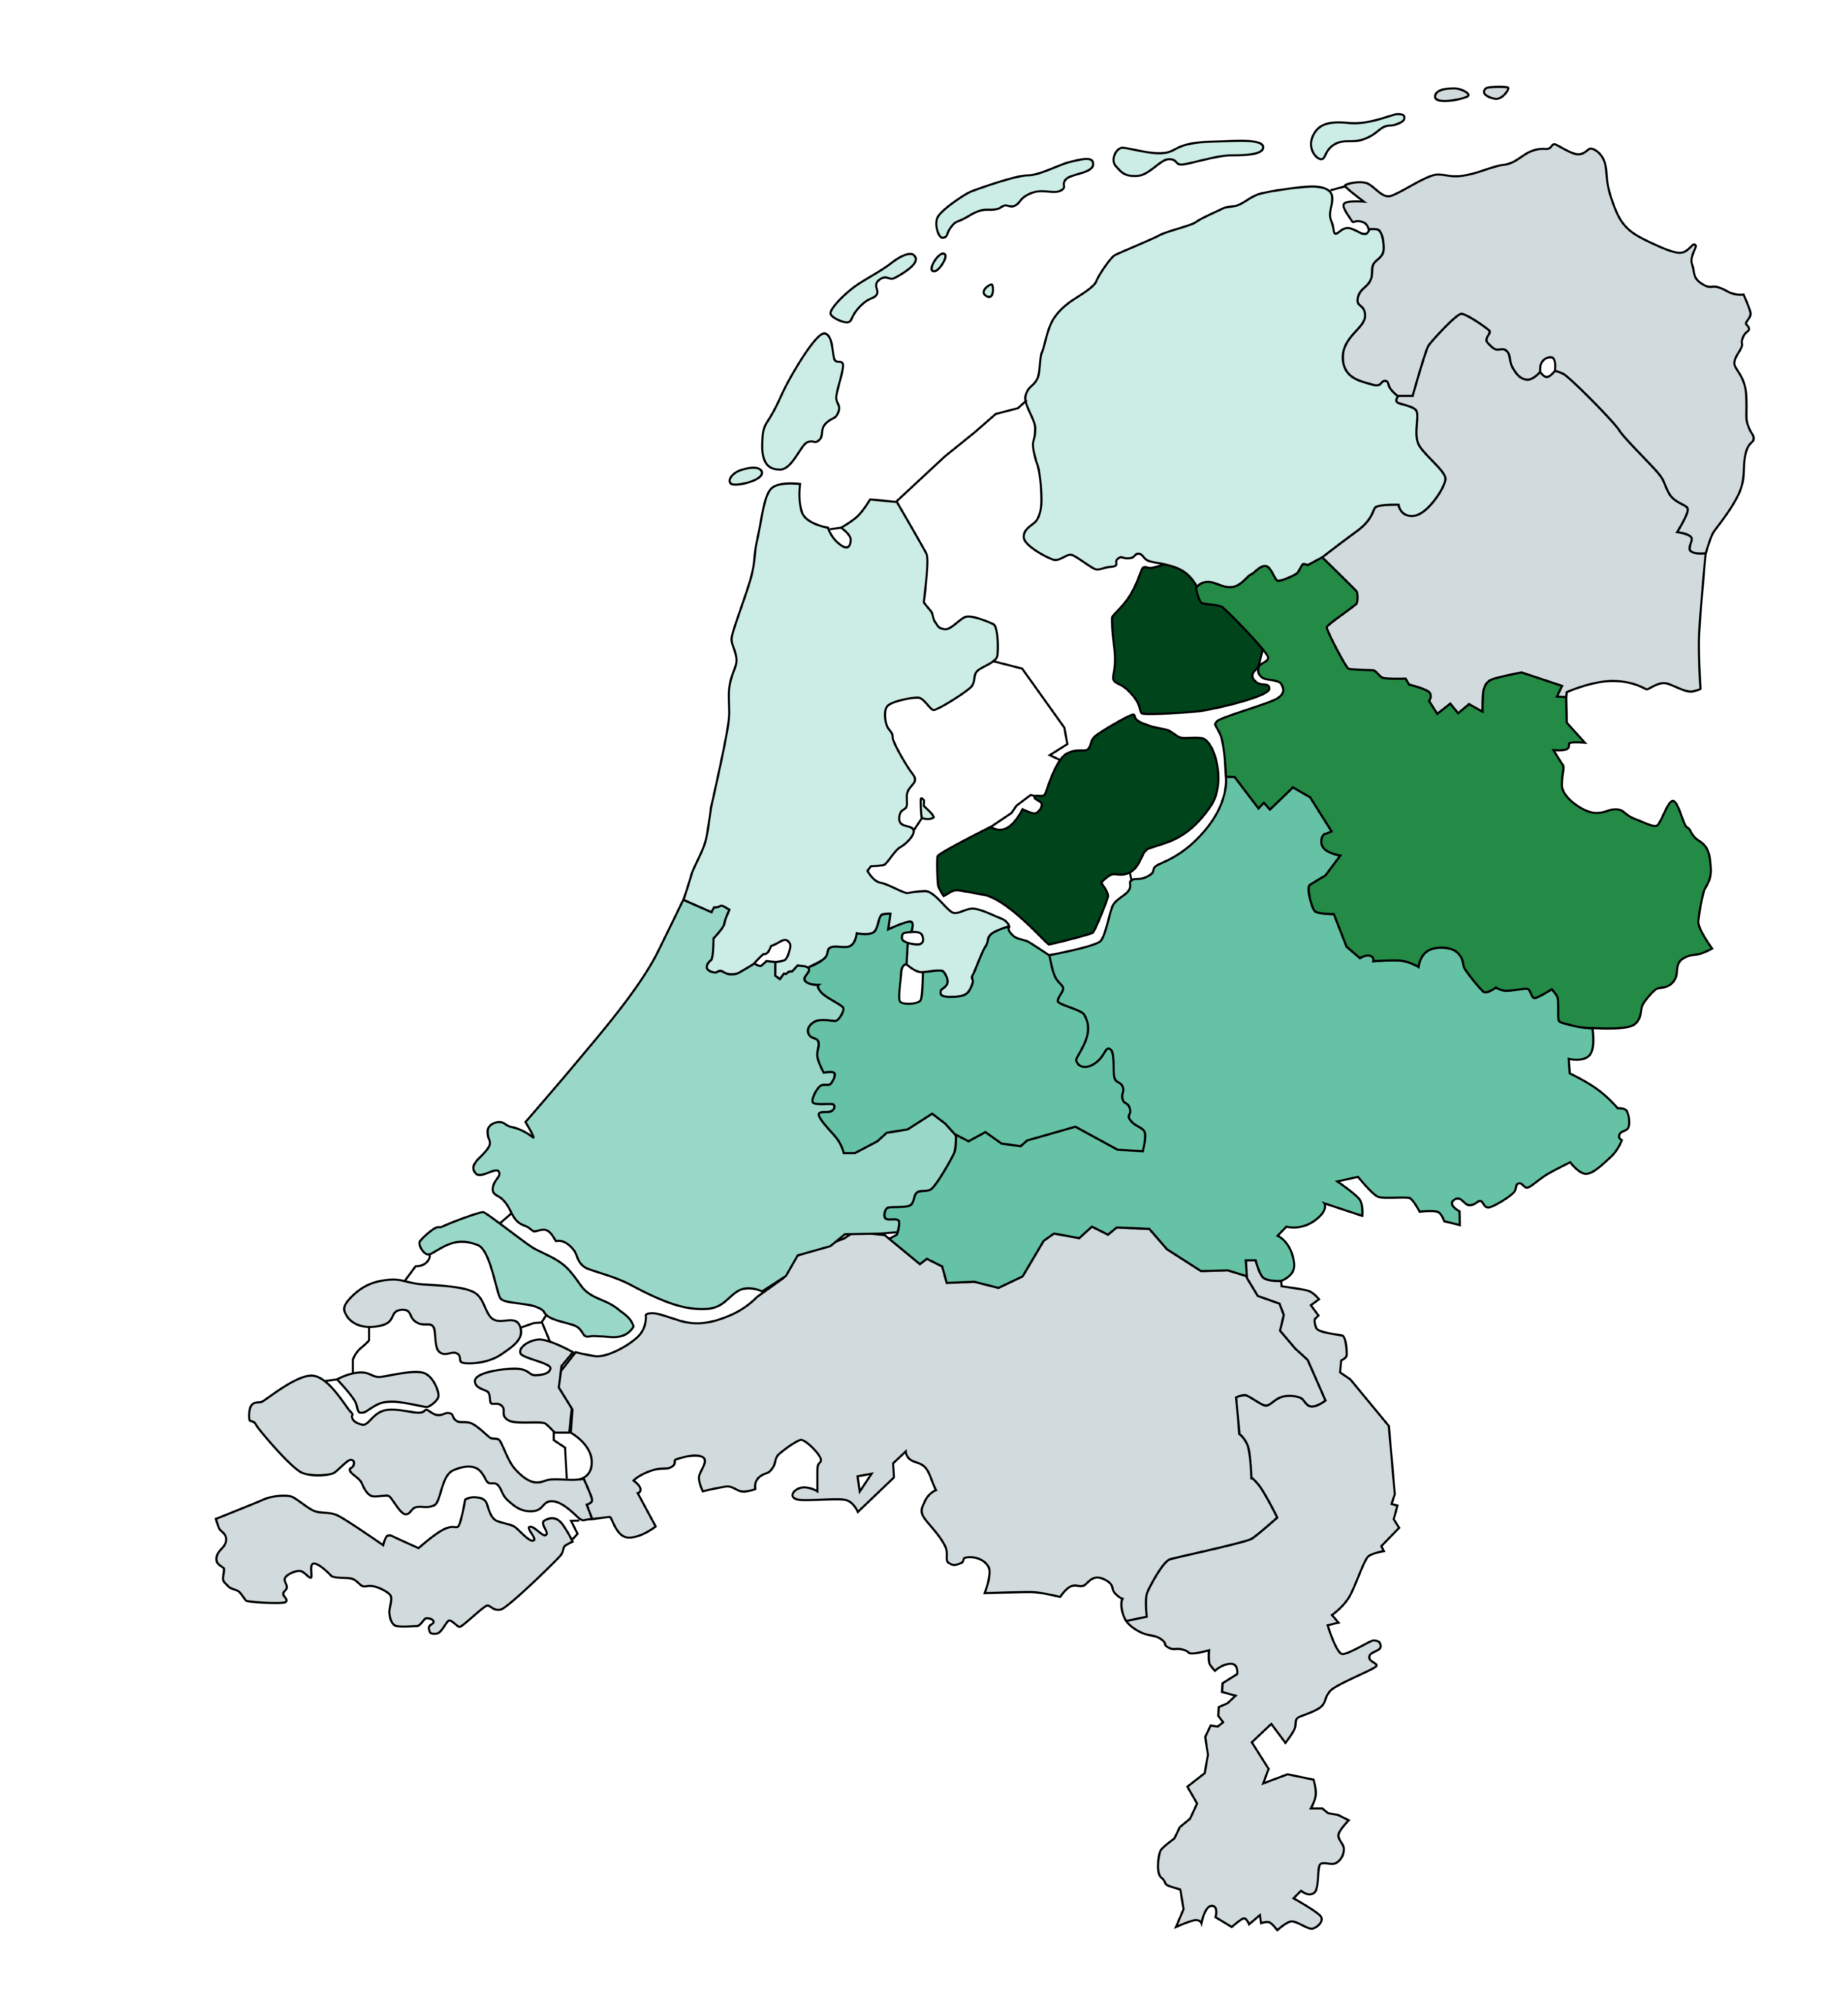
\includegraphics[width=0.66\linewidth]{location-netherlands.png}
		\captionof{figure}{Usage by Dutch Province}
		\label{fig:test2}
	\end{minipage} 
\end{table}

\paragraph{Browsers and Devices} The User-Agent request header is a characteristic string that provides insight into user' browsers and devices, depending on their privacy settings. In Tables 12 and 13, usage by device type and web browser is displayed respectively, with the exception of requests due to uptime monitoring (Section 6.5.1). 

Although Google Chrome is the most popular web browser as reported by Wikimedia in November 2019 [X], it placed behind both Mozilla Firefox and Apple Safari in usage by participants in this research. After Chrome followed the mobile version of Safari and the headless version of Chrome.

\begin{table}[!htb]
	\begin{minipage}{.5\linewidth}
		\caption{Usage by Operating System}
		\centering
		\begin{tabular}{lr}
			\hline
			\textbf{Operating System} & \textbf{Percentage} \\
			\hline
			macOS                     & 49.93\%             \\
			Other Linux               & 26.53\%             \\
			Windows                   & 17.47\%             \\
			Android                   & 2.22\%              \\
			iOS                       & 1.96\%              \\
			Ubuntu                    & 1.89\%              \\
			\hline
		\end{tabular}
	\end{minipage}%
	\hspace{.1cm}
	\begin{minipage}{.5\linewidth}
		\centering
		\caption{Usage by Web Browser}
		\begin{tabular}{lr}
			\hline
			\textbf{Browser}  & \textbf{Percentage} \\
			\hline
			Firefox           & 47.59\%                \\
			Safari            & 30.25\%                \\
			Chrome            & 19.17\%                \\
			Safari (mobile)   & 1.50\%                 \\
			Chrome (headless) & 1.17\%                 \\
			Chromium          & 0.26\%                 \\
			\hline
		\end{tabular}
	\end{minipage} 
\end{table}

\paragraph{Other Analytics}

In terms of the user's browser language, English was the overwhelming majority, detected in over 95\% of all pageviews. This was divided into 65\% US English, 30\% general English, and 2\% British English. Apart from English, 1\% was Dutch and less than 1\% was Polish.

Similarly, over 99\% of all pageviews were done on URLs on the secure HTTPS protocol, with only 4 requests using HTTP. This was due to the secure protocol redirection described in Section 6.2.5.

Most users used the web app a large screen, not a smartphone. In fact, over 30 unique screen resolution combinations were tracked. The most common absolute screen resolution was the high definition 1920x1080 (35\%), followed by 1440x900 at almost a quarter of all pageviews. Interestingly, 2\% of all pageviews still used the outdated 800x600 resolution.

\subsubsection{API usage}

Whenever a participant uses the web app, requests to the API are made. An average of 1,077 API requests were made on each day from June 1 to 10. The number of requests on each day is graphed in Figure 9.

An API endpoint is triggered when a user sends a new email to their assistant, as described in Section 6.2. Unless an error occurs, the assistant responds to each email as well. Figure 10 shows the number of new emails processed every day. The average number of daily emails processed per day was 4.

\begin{figure}
	\centering
	\begin{minipage}{.47\textwidth}
		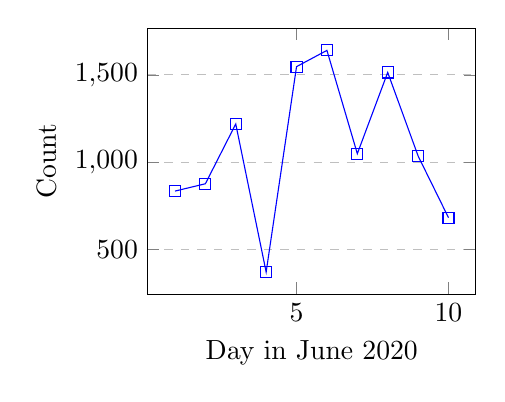
\begin{tikzpicture}
			\begin{axis}[
					width=5.75cm,
					xlabel={Day in June 2020},
					ylabel={Count},
					legend pos=north west,
					ymajorgrids=true,
					grid style=dashed,
				]
				\addplot[
					color=blue,
					mark=square,
				]
				coordinates {
					(1,835)(2,877)(3,1219)(4,372)(5,1547)(6,1640)(7,1049)(8,1514)(9,1036)(10,683)
				};
			\end{axis}
		\end{tikzpicture}
		\caption{Number of API requests received per day}
	\end{minipage}%
	\hspace{.5cm}
	\begin{minipage}{.47\textwidth}
		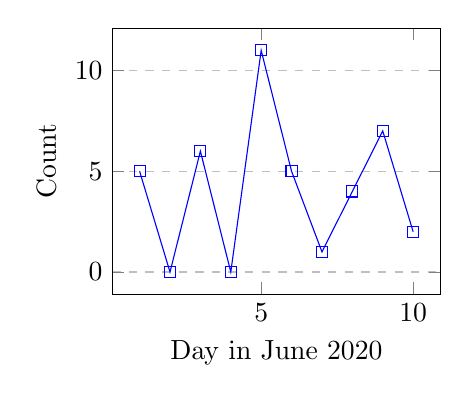
\begin{tikzpicture}
			\begin{axis}[
					width=5.75cm,
					xlabel={Day in June 2020},
					ylabel={Count},
					legend pos=north west,
					ymajorgrids=true,
					grid style=dashed,
				]
				\addplot[
					color=blue,
					mark=square,
				]
				coordinates {
					(1,5)(2,0)(3,6)(4,0)(5,11)(6,5)(7,1)(8,4)(9,7)(10,2)
				};
				
			\end{axis}
		\end{tikzpicture}
		\caption{Number of emails processed per day}
	\end{minipage}
\end{figure}

\subsubsection{Heatmaps}

To better measure how participants used the web app, each mouse click was also tracked. This tracking was completely anonymous, collecting only the details of the component clicked on apart from the datapoints described above, without linking the clicks to a particular user ID.

Heatmaps convey the distribution of attention on a page [X]. A total of 3,271 clicks were tracked and the figures below are presented by superimposing the heatmap over the screenshot of the respective component.

\begin{wrapfigure}{l}{0.45\textwidth}\centering
	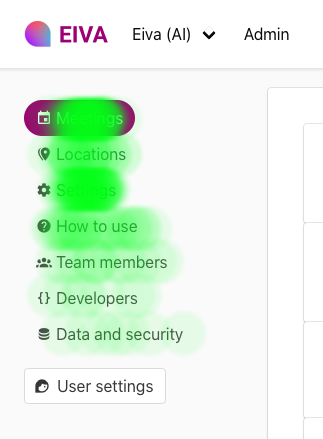
\includegraphics[scale=0.5]{heatmap-sidebar.png}
	\caption{Heatmap for Sidebar}
\end{wrapfigure}

\paragraph{Navigation}

In Figure 11, the distribution of clicks on the sidebar navigation is showcased. This heatmap was generated using 403 datapoints and shows that Settings was clicked on most frequently (106 times), followed in order by Meetings (105), Locations (71), How to use (58), Team members (13), Developers (20), and Data and security (15).

\begin{figure}
  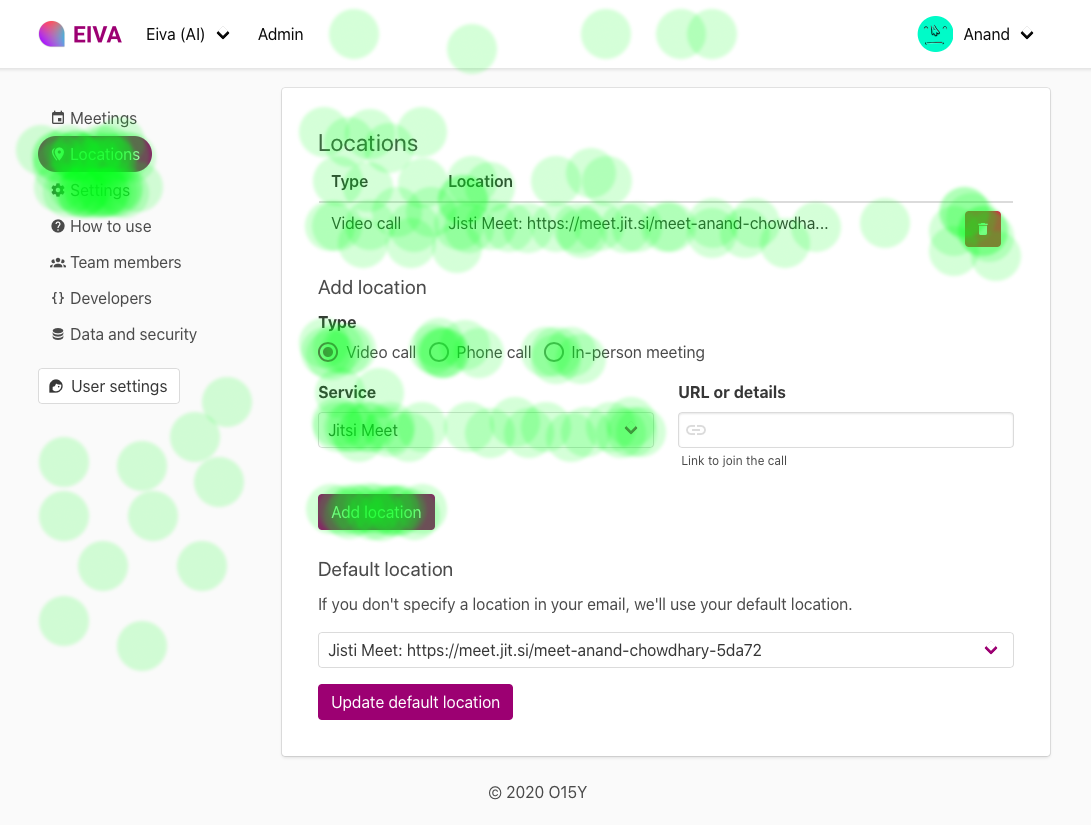
\includegraphics[width=\textwidth]{heatmap-locations.png}
  \caption{Heatmap for Locations Page}
\end{figure}

\paragraph{Webpage}

The Locations page is an ideal example to measure clicks because it has several controls and links. Figure 12, generated with 237 datapoints, shows.

The sidebar navigation on the Locations page has the most frequently clicked item of Settings (19 clicks), which is expected since it is the next link after Locations itself. Users also clicked on the table containing the list of saved locations and the Delete button for each item.

In the Add Locations selector, both Video call and Phone call were selected 6 times, whereas In-person meeting was selected 5 times. The Service dropdown selector was clicked on 24 times. The Add Location button was clicked on 14 times. In this example, the Update default location button in unused because it was added after June 10, 2020.

Overall, it is clear that users interacted with all controls on the webpage --- the sidebar navigation, locations table, buttons, and input fields.

\subsection{User Experience Evaluation}

The first question, \emph{What comes to mind when you think about EIVA; how would you describe it to a friend?}, allows users to share their first impressions after using the service. Some of the responses were:

\begin{enumerate}
	\item ``A smart interface to my calendar"
	\item ``A way to avoid having to talk to people to schedule your appointments with them"
	\item ``Make my appointment very easy, Easy to see all meetings in one screen! Awesome Product!"
	\item ``Interesting personal automation, severely limited at the moment"
\end{enumerate}

\subsubsection{Webapp Experience}

Users were asked to rate the web app on different parameters, from 0 to 5. All parameters scored over 4 out of 5, with privacy features rated with the highest average of 4.9.

\begin{table}[!htb]
	\begin{minipage}{1\linewidth}
		\caption{Webapp Experience Ratings}
		\centering
		\begin{tabular}{llcc}
			\hline
			\textbf{Parameter} & \textbf{Average}   & \textbf{Median} & \textbf{Mode} \\
			\hline
			Overall experience & \score{4.3}{5} 4.3 & 4               & 4             \\
			Design             & \score{4.5}{5} 4.5 & 4               & 5             \\
			Functionality      & \score{4.3}{5} 4.3 & 4               & 4             \\
			Ease of use        & \score{4.2}{5} 4.2 & 4               & 4 \& 5        \\
			Privacy features   & \score{4.9}{5} 4.9 & 5               & 5             \\
			\hline
		\end{tabular}
	\end{minipage}%
\end{table}

\subsubsection{Assistant Experience}

Similarly, users were asked to rate the assistant on different parameters, from 0 to 5.

\begin{table}[!htb]
	\begin{minipage}{1\linewidth}
		\caption{Assistant Experience Ratings}
		\centering
		\begin{tabular}{llcc}
			\hline
			\textbf{Parameter}                         & \textbf{Average}   & \textbf{Median} & \textbf{Mode} \\
			\hline
			Overall experience                         & \score{4.6}{5} 4.6 & 5               & 5             \\
			Customizability                            & \score{4.4}{5} 4.4 & 4               & 5             \\
			Natural language understanding flexibility & \score{4.4}{5} 4.4 & 4               & 5             \\
			Sounding human-like over email             & \score{4.3}{5} 4.3 & 4               & 4             \\
			Trust                                      & \score{3.7}{5} 3.7 & 4               & 4             \\
			Time recommendations                       & \score{2.7}{5} 2.7 & 3               & 3             \\
			\hline
		\end{tabular}
	\end{minipage}%
\end{table}

To participate in the research, users were required to send at least one email to the EIVA for scheduling an appointment. They were free to send multiple emails, and were asked about the number of emails they sent. 4 out of 10 participants sent only one email, while 6 out of 10 sent between 2 and 5 emails.

To find out whether the assistant understood the overall meaning of their email in natural language, participants were asked \emph{Did the assistant understand your email(s) correctly?}. 7 out of 10 participants responded in the affirmative, while 3 out of 10 responded with `Partially'. No participants responded in the negative, suggesting that the EIVA did a well-enough job understanding incoming emails.

\begin{table}[!htb]
	\begin{minipage}{.5\linewidth}
		\caption{Number of Emails Sent}
		\centering
		\begin{tabular}{lr}
			\hline
			\textbf{Number} & \textbf{Percentage} \\
			\hline
			1               & 40\%                \\
			Between 2 and 5 & 60\%                \\
			More than 5     & 0\%                 \\
			\hline
		\end{tabular}
	\end{minipage}%
	\hspace{.1cm}
	\begin{minipage}{.5\linewidth}
		\centering
		\caption{Correctly Understood}
		\begin{tabular}{lr}
			\hline
			\textbf{Response} & \textbf{Percentage} \\
			\hline
			Yes               & 70\%                \\
			Partially         & 30\%                \\
			No                & 0\%                 \\
			\hline
		\end{tabular}
	\end{minipage} 
\end{table}

Apart from understanding the meaning of an email, participants were asked whether the EIVA recommended the correct location for the meeting. The location recommendation was correct for 7 out of 10 participants.

They were also directly asked whether the EIVA met their expectation in terms of scheduling an appointment. All participants responded positively.

\begin{table}[!htb]
	\begin{minipage}{.5\linewidth}
		\caption{Location Recommendation}
		\centering
		\begin{tabular}{lr}
			\hline
			\textbf{Accurate} & \textbf{Percentage} \\
			\hline
			Correct           & 70\%                \\
			Incorrect         & 30\%                \\
			\hline
		\end{tabular}
	\end{minipage}%
	\hspace{.1cm}
	\begin{minipage}{.5\linewidth}
		\centering
		\caption{EIVA Met Expectations}
		\begin{tabular}{lr}
			\hline
			\textbf{Response} & \textbf{Percentage} \\
			\hline
			Yes               & 100\%               \\
			No                & 0\%                 \\
			\hline
		\end{tabular}
	\end{minipage} 
\end{table}

\subsubsection{Business Case}

Since the big picture goal of the client is to launch EIVA as a paid service, participants were asked whether they would use EIVA on launch. 8 out of 10 participants said that they would, whereas 2 out of 10 wouldn't.

Participants were also asked how much they would be willing to pay every month for such as service. 4 out of 10 participants said that the service should be free, 3 out of 10 would each pay €5 or less, or €10 or less, per month. No participants wanted to pay €20 per month.

\begin{table}[!htb]
	\begin{minipage}{.5\linewidth}
		\caption{Would Use EIVA}
		\centering
		\begin{tabular}{lr}
			\hline
			\textbf{Accurate} & \textbf{Percentage} \\
			\hline
			Yes               & 80\%                \\
			No                & 20\%                \\
			\hline
		\end{tabular}
	\end{minipage}%
	\hspace{.1cm}
	\begin{minipage}{.5\linewidth}
		\centering
		\caption{Monthly Subscription Fees}
		\begin{tabular}{lr}
			\hline
			\textbf{Response} & \textbf{Percentage} \\
			\hline
			€0              & 40\%                \\
			€5 or less      & 30\%                \\
			€10 or less     & 30\%                \\
			\hline
		\end{tabular}
	\end{minipage} 
\end{table}

\subsubsection{Final Impressions}

Respondents could optionally add additional information in the form of long-form answers. A selection of answers is listed below.

\begin{enumerate}
	\item Did you find anything frustrating that you wish was easier or different?
	      \begin{enumerate}
	      	\item Support BCC instead of CC in emails
	      	\item The onboarding tour is too long
	      \end{enumerate}
	\item Is there anything that you wish the assistant could do, in terms of scheduling, that it doesn't currently?
	      \begin{enumerate}
	      	\item Cancel or reschedule via online interface
	      	\item Send an email at a set time every day about my day's schedule
	      \end{enumerate}
	\item What do you like the most about EIVA?
	      \begin{enumerate}
	      	\item Simplicity and ease of use
	      	\item Saving back and forth emailing during scheduling
	      	\item Fast, secure, and nice user interface
	      	\item Virtual tutor at every point to choose the next right option
	      	\item Natural language understanding
	      	\item Human-like conversational emails
	      \end{enumerate}
	\item What do you like the least about EIVA?
	      \begin{enumerate}
	      	\item Pretending to be human
	      	\item Lengthy and slightly technical onboarding process
	      \end{enumerate}
	\item Do you have any additional feedback, suggestions, or comments?
	      \begin{enumerate}
	      	\item I am thrilled with my first experience in using an assistant
	      	\item Add support for hardware authentication
	      \end{enumerate}
\end{enumerate}

\newpage

\section{Conclusion}

...7 out of 10 prefer using email for scheduling...

\newpage

\section{Future Work}

\subsection{Business Case}

In the literature research for this paper, it is highlighted that professionals currently either schedule appointments themselves or hire assistants to help with the task. However, regardless of whether the professional or their assistant schedules appointments, the time wasted is not insignificant. According to the European Commission, the average Dutch small or medium-sized enterprise (SME) employs 3.2 people \cite{noauthor_2019_2019}. If each employee attends 7 meetings per week (which is the average for professionals), 26 otherwise productive hours are wasted every month in scheduling meetings \cite{kincaid_electronic_1985}. This costs the company over €450 in lost time, based on the average wage of €17.6 per hour \cite{noauthor_salary_nodate} This adds up to almost €2.25 billion per year for the SME industry as a whole, and the numbers are even higher for larger enterprises. University of Twente, for example, employs 3,150 professionals, adding up to over €400,000 in lost time per year.

Therefore, a strong business case can be built around launching EIVA as a service. Since the assistant can save around €150 in lost time per month for professionals, a service that costs as high as €100 per month per person has a return on investment (ROI) of 50\%. In my personal opinion, a pricing point of less than €50 per month can be achieved because of the low cloud infrastructure costs. The proposed pricing plans are:

\begin{enumerate}
	\item Basic plan for €10 per month, targeted towards students, self-employed young professionals, and early-stage entrepreneurs with no support for custom domain, but including unlimited scheduling and assistant usage
	\item Pro plan for €25 per month with support for custom domain
	\item Team plan for €30 per user per month, targeted towards businesses or institutions who want to onboard their entire team to EIVA for a collaborative experience
	\item Custom plan with custom billing for large enterprises with features like dedicated support, on-premise hosting, and uptime service-level agreements (SLA)
\end{enumerate}

\newpage

\cleardoublepage
\pagenumbering{roman}
\setcounter{page}{\thesavepage}

\section*{Appendix 1: Information Brochure}

If you want to get in touch with the researchers, client, or supervisor, you can find their details below. If you have any queries, complaints, or comments about this research, you can contact the Secretary of the Ethics Committee.

\paragraph{Research Leader}
Anand Chowdhary\newline
Address: Roerstaart 28, 7543AC Enschede, the Netherlands\newline
Phone: +31 0 644691056\newline
Email: a.chowdhary@student.utwente.nl

\paragraph{Research Client}
Speakup B.V.\newline
Address: Institutenweg 6, 7521PK Enschede, the Netherlands\newline
Phone: +31 0 887732587\newline
Email: info@speakup.nl

\paragraph{Research Supervisor}
dr. Job Zwiers\newline
Address: Zilverling 1060, 7522NH Enschede, the Netherlands\newline
Phone: +31 0 534893816\newline
Email: j.zwiers@utwente.nl

\paragraph{Secretary of the Ethics Committee}
drs. Petri de Willigen\newline
Address: Zilverling 1051, 7522NH Enschede, the Netherlands\newline
Phone: +31 0 534892085\newline
Email: ethics-comm-ewi@utwente.nl

\paragraph{Purpose}

Scheduling appointments manually can waste a lot of time, and our goal is to provide you with a virtual assistant that can automate the process of scheduling based on your preferences and availability. This research will help us understand the accuracy of the assistant, the end user experience, and whether or not end users will use it when we launch it as a service.

\paragraph{Research Procedure}

After you have signed the Consent Form and answered some questions, you can register for the virtual assistant service on the website. An onboarding interface will help you set up your account, connect your calendar, and set up your scheduling preferences (such as working days, meeting locations, and preferred times). After using the virtual assistant to schedule at least one meeting, you can continue to fill this survey about your experience. Apart from your survey response, computed data such as how long it takes the assistant to set up your appointment and analytics about your usage of the web application will also be collected and aggregated. Once the research is over, you can choose to receive a copy of the results.

\paragraph{10 Minutes}

It will takes around 10 minutes to complete this survey, including interacting with your virtual assistant. It is recommended to use a laptop, tablet, or desktop computer. If none of these are available to you, you can also use a smartphone. After you have submitted this form, you can continue to use the virtual assistant service, if you choose to, but only the usage within the research period will be measured.

\paragraph{Remuneration}

This research is voluntary and there is no monetary compensation for participation. However, after this research has ended, this virtual assistant service will launch as a paid subscription service for professionals. As a research participant, you will receive €100 in service credits or equivalent, and a coupon code will be emailed to you at the end of this research.

\paragraph{Anonymous}

Anonymity will be guaranteed to all participants, and your individual data will not be disclosed to third parties without your explicit permission. Furthermore, the data obtained from this research is not published in any way that would make it possible to link the results or other findings with a particular subject. Only aggregated or anonymized data will be published.

\paragraph{Voluntary}

Participation remains at all times voluntary and you may refuse to participate in this research at any time, without giving any reason. You can also refuse that we use your data for the research within 24 hours of completing the survey. There is no specific category of persons who are advised not to participate in the research due to an increased level of risk or discomfort.

\paragraph{COVID-19 Note}

This research is completely online and based on your usage of a web application, sending emails, and answering a survey. At no point will participants be asked to interact with a physical installation or answer questions in person. It is recommended that you participate from the comfort of your home. There is no possibility of accidental discoveries in this research.

\newpage

\section*{Appendix 2: Consent Form}

This section ensures that we have your permission to conduct this research. Please note that participation remains at all times voluntary and you may refuse to participate in this research at any time, without giving any reason.

\begin{enumerate}
	\item Before we sign you up for this research, we need to make sure that you can give us permission. Note that you are not eligible for this research if you are under the age of 18 or otherwise incapable of giving us your informed consent. I am above the age of 18 and capable of giving informed consent.
	\item In this research, you will use a virtual assistant web application and communicate with the assistant over email. You will have to answer a series of questions about your experience using the application and communicating with the assistant. By checking ``I agree", you permit us to use the data from your answers for purposes of this research.
	\item Optional: To find available meeting slots in your agenda, the virtual assistant will require access to your calendar. To allow access, you can add a link to your calendar using the web app. You can also remove access at any time. By checking ``I agree", you permit us to have read-only access to your calendar.
	\item In order to use the web application, you provide your personal information such as your name and email address. Optionally, you can also add your phone numbers and office addresses to allow the virtual assistant to schedule in-person meetings or phone calls. By checking ``I agree", you permit us to store this information and use it for scheduling appointments.
	\item Your usage of the web application will be analyzed in the background, such as how long it takes you to complete the onboarding flow and to set up an appointment using the assistant. This data will be only be collected anonymously and published after aggregation. By checking ``I agree", you permit this data collection.
	\item Under the General Data Protection Regulation, we need your permission to store your information on our servers. You can export a copy of all your data or permanently delete it at any time from the web application. By selecting an option, you permit us to store your information.
\end{enumerate}

\newpage

\section*{Appendix 3: Code Repositories}

All code written for this project is open-source, available on GitHub:

\begin{enumerate}
	\item Backend APIs: \url{https://github.com/o15y/eiva}
	\item Frontend web application: \url{https://github.com/o15y/myeiva.com}
	\item Companion open-source packages:
	      \begin{enumerate}
	      	\item Calendar Slots: \url{https://github.com/AnandChowdhary/calendar-slots}
	      	\item Calendar Link: \url{https://github.com/AnandChowdhary/calendar-link}
	      	\item Staart API: \url{https://github.com/staart/api}
	      	\item Staart UI: \url{https://github.com/staart/ui}
	      \end{enumerate}
\end{enumerate}

\newpage

\section*{Appendix 4: Open Source Licenses}

This project is standing on the shoulder of giants; it wouldn't be possible without the open source projects listed below. Only direct NPM dependencies are listed below (not development dependencies or subdependencies).

\subsection*{Backend}

\paragraph{MIT License} @staart/config, @staart/disposable-email, @staart/elasticsearch, @staart/errors, @staart/mail, @staart/messages, @staart/mustache-markdown, @staart/payments, @staart/redis, @staart/scripts, @staart/server, @staart/text, @staart/validate, axios, calendar-link, calendar-slots, chrono-node, cron, fs-extra, geolite2-redist, jsonwebtoken, mailparser, maxmind, moment, moment-timezone, mysql, natural, node-email-reply-parser, node-emoji, otplib, qrcode, random-int, systeminformation

\paragraph{Apache 2.0} @prisma/cli, @prisma/client, client-oauth2, googleapis, snyk

\paragraph{Other} randomcolor (CC0), email-signature-detector (ISC), @sentry/node (BSD 3 Clause)

\subsection*{Frontend}

\paragraph{MIT License} @nuxtjs/axios, @nuxtjs/pwa, analytics-icons, countries-and-timezones, js-file-download, jwt-decode, nuxt, nuxt-buefy, shepherd.js, ua-parser-js, unique-selector, vue-stripe-elements-plus, vuex-persist

\paragraph{Other} @sentry/browser (BSD 3 Clause)

\newpage

\section*{Appendix 5: Prisma Database Schema}

\subsection*{Enumerated types}

Enumerated types (ENUMs) are a data type consisting of a set of named values. In the Prisma database schema, the following custom-defied ENUMs are used.

\begin{multicols}{2}
	\begin{verbatim}
enum Gender {
  MALE
  FEMALE
  NONBINARY
  UNKNOWN
}

enum NotificationEmails {
  ACCOUNT
  UPDATES
  PROMOTIONS
}

enum PrefersColorScheme {
  NO_PREFERENCE
  LIGHT
  DARK
}

enum PrefersReducedMotion {
  NO_PREFERENCE
  REDUCE
}

enum UserRole {
  SUDO
  USER
}

enum MembershipRole {
  OWNER
  ADMIN
  RESELLER
  MEMBER
}

enum MeetingType {
  IN_PERSON
  PHONE_CALL
  VIDEO_CALL
}

enum EmailStatus {
  PENDING
  SUCCESS
  ERROR
}

enum EmailType {
  INCOMING
  OUTGOING
}
	\end{verbatim}
\end{multicols}

\subsubsection*{Entire Schema}

The full schema was omitted from this appendix because it is 357 lines. It is available in the `prisma' directory part of the backend source code, on \url{https://github.com/o15y/eiva/blob/master/prisma/schema.prisma}.

\newpage

\bibliography{citations}

\paragraph{License} This work is licensed under a Creative Commons Attribution 4.0 International License (CC BY 4.0). The source code of this research paper is available on \url{https://github.com/AnandChowdhary/thesis}.

\end{document}